% ============================================================================
% main.tex  --  Minimum wages and workers by education level in Peru
% Compiles with pdflatex + bibtex (author-year via natbib/apalike), or tectonic.
%   pdflatex main ; bibtex main ; pdflatex main ; pdflatex main
% ============================================================================
\documentclass[12pt]{article}

\usepackage[utf8]{inputenc}
\usepackage[T1]{fontenc}
\usepackage{lmodern}
\usepackage[english]{babel}
\usepackage{amsmath,amssymb,amsthm}
\usepackage{graphicx}
\usepackage{booktabs}
\usepackage{threeparttable}
\usepackage{caption}
\usepackage{subcaption}
\usepackage{float}
\usepackage[margin=1in]{geometry}
\usepackage{setspace}
\usepackage[authoryear,round]{natbib}
\bibliographystyle{apalike}
\usepackage[hidelinks]{hyperref}
\usepackage{xcolor}
\usepackage{siunitx}
\usepackage{enumitem}

\captionsetup{font=small,labelfont=bf}
\setlength{\parskip}{2pt}
\graphicspath{{figures/}{figures/}}

\newcommand{\Low}{\mathrm{Low}}
\newcommand{\Post}{\mathrm{Post}}

\title{\textbf{Shifting, Not Lifting:\\
Minimum Wages, Informality, and Low-Skilled Workers in Peru}\thanks{This paper uses the public-use quarterly
employment modules of the Encuesta Nacional de Hogares (ENAHO) of the Instituto
Nacional de Estadística e Informática (INEI). All estimates use survey weights;
the replication package is available in the accompanying repository. All errors are
the author's own.}}

\author{Eric Torres Ramirez\\
  \small Pontificia Universidad Católica del Perú\\
  \small \texttt{etorresram@gmail.com}}
\date{This version: \today}

\begin{document}
\maketitle

\begin{abstract}
\noindent
Whether a minimum wage helps the workers it targets depends on how many of them it
reaches, and on whether anyone complies with it. I study Peru's May 2022 increase in
the national minimum wage, from 930 to 1,025 soles. Peru sets a single national floor,
so identification comes from differential exposure: on the eve of the reform a majority
of low-education wage earners were paid below the new minimum, against two fifths of
the high-education comparison group. Using quarterly ENAHO data (2021--2024), I find
that the reform did not lift the pay of the workers it targeted, even though the floor
was honored where enforcement reaches: within the formal sector the earnings spike at
the old minimum migrates almost completely to the new one, but formal jobs account for
only 13 percent of low-education employment, informal pay drifted further below the
floor, and relative wages did not rise. What moved was the composition of employment:
formal employment of low-education workers fell by 4.6 percentage points, a fifth of
its baseline, and self-employment rose by 3.6 points, with flat pre-reform trends,
larger shifts in high-bite departments, and confirmation from a continuous
regional-exposure design under randomization inference. An identically sized increase
in January 2025, in a calmer labor market, produced no comparable reallocation. Where
informality is pervasive and enforcement weak, minimum wage increases shift low-skilled
workers across employment arrangements more than they raise their pay, qualifying the
``lighthouse'' view of the Peruvian minimum wage found for earlier reforms.

\medskip
\noindent\textbf{Keywords:} minimum wage; informality; education; difference-in-differences; Peru.\\
\noindent\textbf{JEL codes:} J23, J31, J38, J46, O17.
\end{abstract}

\newpage
\onehalfspacing

\section{Introduction}\label{sec:intro}

Whether a minimum wage helps the workers it targets depends on how many of them it actually
reaches. In developing countries a large share of employment lies outside the reach of labor
regulation, so a statutory wage floor can raise pay for covered workers, displace some of
them into the uncovered informal sector, or act only as a reference point for wages that
formal firms would have paid in any case. Which of these forces dominates is an empirical
question, and its answer turns on how binding the floor is, how well it is enforced, and how
freely workers move between the formal and informal margins. I study these questions for
Peru, a country that pairs a minimum wage high relative to median pay with one of the highest
rates of labor informality in Latin America.

I exploit the increase in Peru's national minimum wage (the \emph{Remuneración Mínima
Vital}, or RMV) from 930 to 1,025 soles, enacted by Supreme Decree 003-2022-TR and effective
on 1 May 2022. This 10.2 percent nominal increase was the first change to the RMV in four
years, and it occurred as the labor market was emerging from the pandemic. A central
institutional fact shapes the analysis: Peru sets a single national minimum wage, with no
regional or sectoral variation in the general regime. There is therefore no cross-sectional
variation in the level of the policy and no staggered adoption to exploit. As
\citet{jimenez_2023} notes for the 2016 reform, credible identification must instead come
from differential \emph{exposure} to a policy that changes for everyone at the same time.

My source of differential exposure is education. In the pre-reform quarters the median
monthly-equivalent wage of a low-education private wage earner was 950 soles, almost exactly
the old minimum of 930, and 57 percent of low-education wage earners were paid below the
\emph{new} floor of 1,025 soles on the eve of the reform; a ten percent increase in that
floor is therefore highly binding for this group. High-education workers, by contrast, have
a median wage well above the minimum and are less likely to be bound by it, although a
substantial minority remains exposed through informal or own-account work. This gap in exposure, rather than a claim of zero
exposure for the comparison group, motivates a difference-in-differences design that
contrasts low-education workers (those with at most complete secondary schooling, about two
thirds of the working-age population) with high-education workers (those with any tertiary
schooling). The design applies a long tradition of measuring minimum wage effects from
variation in the ``bite'' of the policy across groups or regions \citep{card_1992, lee_1999,
machin_manning_rahman_2003} to a setting with a single national reform and rich, quarterly
household data.

I use the public-use quarterly employment modules of the Encuesta Nacional de Hogares (ENAHO)
from 2021Q1 through 2024Q4, which bracket the reform with five pre-reform and ten clean
post-reform quarters; the transition quarter 2022Q2, in which the reform took effect
mid-quarter, is excluded from the baseline and restored in a robustness check. The data are repeated cross-sections, and their quarterly
frequency lets me estimate a dynamic event study, test for differential pre-trends by
education, and trace the effect for more than two years after the reform. I examine a broad
set of outcomes: real hourly wages and monthly earnings, the probability of employment and of
labor force participation, the incidence of formal versus informal employment, hours of work,
and the split of employment between wage work and self-employment. Throughout I weight by the
survey weights and cluster inference by department, and because treatment is assigned at a
coarse level I complement conventional cluster-robust standard errors with the small-sample
correction of \citet{pustejovsky_tipton_2018} and with randomization inference.

Three findings emerge. First, and most robustly, the reform shifted the \emph{composition}
of low-education employment away from formal wage work. The probability that a low-education
worker holds formal employment falls by 4.6 percentage points, about a fifth of the group's
23 percent baseline formality rate, and self-employment rises by 3.6 points. These estimates
have pre-reform formality trends that pass their joint test, with a small residual
drift that I quantify and adjust for; they appear immediately after the
reform and persist, are larger in the departments where the new floor cuts deeper into the
wage distribution, and are confirmed by an independent continuous-exposure design that
relates outcomes to the pre-reform regional Kaitz index and supports design-based
randomization inference. Linked persons in the ENAHO Panel 2020--2024 reveal the flow
behind the stock: incumbent formal workers were retained, while the rate at which
informal low-educated workers entered formal jobs fell by nearly half, so the
reallocation operated through the creation of formal matches rather than their
destruction. Second, there is no evidence that the reform lifted the group's pay, but not because
the floor is a dead letter. Within the formal sector, where enforcement operates, the
earnings spike at the old minimum migrates almost completely to the new one, and the
share of formal wage earners paid below the new floor falls; among informal wage
earners that share \emph{rises}, and because only 13 percent of employed low-education
workers are formal, the two responses cancel: the aggregate below-floor share does not
move, no decile of the wage distribution shows a gain, and the estimated effect on the
average log real hourly wage is negative and insignificant. The no-lift conclusion
rests on the compliance and distributional evidence, whose diagnostics are clean; the
average wage regression itself carries a rejected pre-trend test, driven by a single
early-2021 quarter, and I am explicit about what it can and cannot rule out. Third, the employment
rate of low-education workers falls by 2.5 percentage points, but this margin is the least
robust: it fails in-time placebo tests, has a clear differential pandemic-recovery
pre-trend, and does not scale with regional exposure, so I do not give it a causal
interpretation. Throughout I bound conclusions with the sensitivity analysis of
\citet{rambachan_roth_2023} and a battery of specification and placebo checks. I then
replicate the whole design on the January 2025 reform, which raised the RMV to 1,130 soles
in a calmer, post-pandemic window: no wage response appears there either, and neither does
the reallocation, which I interpret as evidence that the margin along which the minimum
wage binds depends on the state of the labor market.

The contribution is a combination rather than a new tool, and I state it without overclaiming.
To my knowledge this is the first evaluation of the 2022 Peruvian minimum wage reform and
the first study of any Peruvian reform using the post-pandemic quarterly ENAHO; the existing
micro evidence stops at the 2016 reform \citep{jimenez_2023} or at the reforms of the early
2000s \citep{jaramillo_lopez_2006, cespedes_2005}. It is also the first to make heterogeneity
by education the central object of a worker-level event study of the Peruvian minimum wage,
where prior work cuts heterogeneity by income range or age or constructs a department-level
dose of exposure. It is, to my knowledge, also the first to use the linked ENAHO Panel to
measure worker-level formality transitions around any Peruvian minimum wage reform, which
lets me separate the retention of incumbents from the entry of new workers into formal
jobs. And it places the informal margin at the center of the analysis, showing
that adjustment runs through the composition of employment rather than through pay. I claim no
novelty for the identification idea, which is the standard exposure or bite design, nor for
the econometric toolkit; the value added is the pairing of a new reform and a policy-relevant
post-pandemic period with an education-based worker-level design and a careful treatment of
informality and of the threats to identification that such a design entails.

The rest of the paper proceeds as follows. Section~\ref{sec:institutional} describes the
Peruvian minimum wage and the reform, and Section~\ref{sec:literature} places the paper in the
literature. Section~\ref{sec:data} presents the data and the construction of the key
variables, and Section~\ref{sec:strategy} sets out the empirical strategy and the identifying
assumptions. Section~\ref{sec:results} reports the main results, Section~\ref{sec:robustness}
the robustness and inference checks, and Section~\ref{sec:heterogeneity} the heterogeneity and
distributional analysis. Section~\ref{sec:discussion} discusses mechanisms, external validity,
and limitations, and Section~\ref{sec:conclusion} concludes.

\section{Institutional background}\label{sec:institutional}

\subsection{The Peruvian minimum wage}

Peru sets a single national minimum wage, the \emph{Remuneraci\'on M\'inima Vital}
(RMV), which applies to workers in the private-sector labor regime. Unlike federal
systems such as the United States or Brazil, and unlike countries with occupational
or regional wage floors, Peru has no sub-national or industry-specific statutory
minimum in the general regime. A small number of activities carry fixed multiples of
the RMV (for example the mining premium and the agricultural daily wage), but these
are pegged mechanically to the national value and move with it. The consequence for
research design is decisive: because the level of the RMV is common to the whole
country, there is no cross-sectional variation in the policy and no staggered timing
of adoption. Any credible research design must therefore exploit differences in how
exposed workers are to a change that reaches everyone simultaneously.

In principle the RMV is to be adjusted periodically by the tripartite National Labor
Council in line with inflation and productivity. In practice the Council has never
set the RMV, and the level is fixed at the discretion of the executive through a
Supreme Decree. Adjustments are consequently infrequent and irregular in both timing
and magnitude, and Peru is among the most volatile minimum wage setters in the
region \citep{jimenez_2023, cespedes_2005}. The RMV had stood at 930 soles since
April 2018.

Two features make the RMV unusually binding by international standards. First, its
ratio to the median wage is high. In our pre-reform sample the national median
monthly wage of a dependent employee is almost exactly 930 soles, so the old minimum
already sat at the median of the covered wage distribution and the Kaitz index, the
ratio of the minimum to the median wage, is close to one nationally and well above
one in the poorer departments. Second, compliance is far from universal. Consistent
with earlier work \citep{jaramillo_lopez_2006, cespedes_2005}, a large share of
workers earn below the statutory floor, especially in rural areas, in small firms,
and in the informal sector, while compliance inside registered formal firms is high.
Enforcement capacity is limited. These features imply that a nominal increase in the
RMV can bind mechanically for formal workers near the floor while leaving much of the
informal sector formally uncovered, so that the policy's real reach depends on the
degree of informality and on the ease of movement across the formal and informal
margins.

\subsection{The 2022 reform}

The reform we study was enacted by Supreme Decree 003-2022-TR, signed on 2 April 2022
and published on 3 April, and took effect on 1 May 2022. It raised the RMV from 930
to 1,025 soles, an increase of 95 soles or 10.2 percent, the first change in four
years. Figure~\ref{fig:mw} plots the nominal and real value of the RMV over
2021--2025. Two points are worth noting. The nominal increase of 10.2 percent was
partly offset by inflation, which ran at roughly 8 percent over 2022, so the increase
in the real value of the floor was more modest and eroded over the following two
years. This tempers the expected size of any wage response and is relevant when
comparing our estimates with those from lower-inflation episodes. The reform also
occurred during the post-pandemic recovery, a period of unusual labor market
turbulence that we address explicitly in the empirical analysis.

A second reform, enacted by Supreme Decree 006-2024-TR and effective on 1 January
2025, raised the RMV further to 1,130 soles. This change falls just outside our main
study window, but the ENAHO quarters for 2025 are available and we use this second
reform as an out-of-sample replication of the design in Section~\ref{sec:robustness}.
The two reforms are of very similar magnitude, 10.2 percent each, which makes the
2025 episode a natural validation exercise in a calmer, post-pandemic environment.

\begin{figure}[H]
\centering
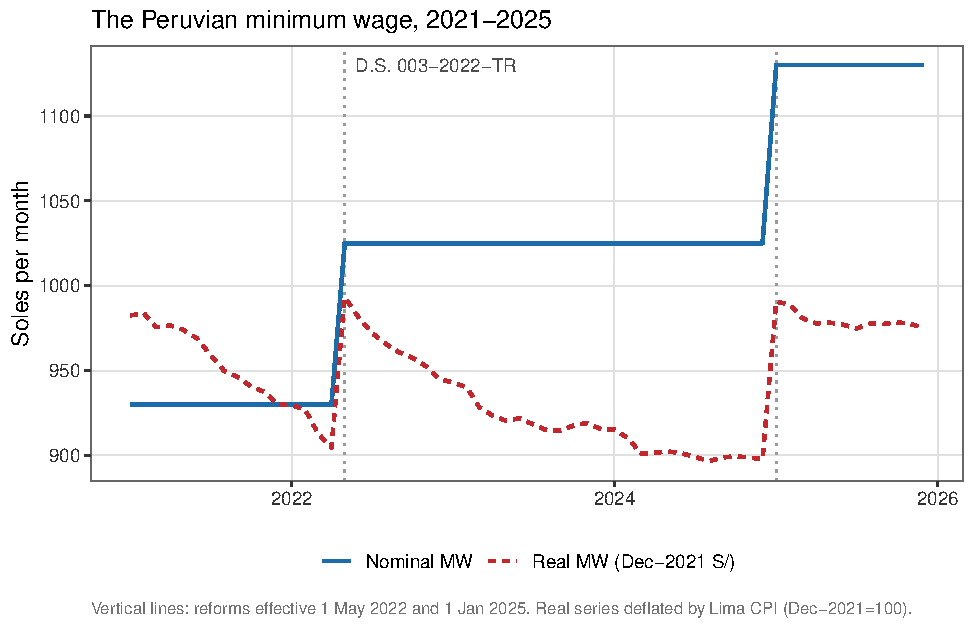
\includegraphics[width=0.82\textwidth]{fig1_minimum_wage.pdf}
\caption{The nominal and real Peruvian minimum wage, 2021--2025. The real series is
deflated by the Lima consumer price index (December 2021 = 100). Vertical dotted
lines mark the reforms effective 1 May 2022 (Supreme Decree 003-2022-TR) and 1
January 2025 (Supreme Decree 006-2024-TR).}
\label{fig:mw}
\end{figure}

\section{Related literature}\label{sec:literature}

My paper connects three strands of research: the theory and evidence on minimum
wage employment effects, the evidence for developing countries with large informal
sectors, and the specific literature on Peru.

\paragraph{Theory and the canonical evidence.} The competitive model predicts that a
binding wage floor reduces employment among low-productivity workers, with an effect
whose size depends on labor demand elasticities and on the fraction of workers bound
by the floor \citep{brown_1999}. Models with employer wage-setting power deliver
different predictions: under monopsony a moderate minimum wage can raise employment,
and it typically compresses the lower tail of the wage distribution
\citep{manning_2003}. The empirical literature has moved from a presumption of sizable
disemployment toward a consensus of small effects on the margin studied. The case
study of \citet{card_krueger_1994} and the broader synthesis in \citet{card_krueger_1995}
found little evidence of job loss from the New Jersey reform, and the border-discontinuity
design of \citet{dube_lester_reich_2010} and the bunching approach of
\citet{cengiz_2019} likewise find that recent United States increases raised wages at
the bottom with limited employment effects. \citet{harasztosi_lindner_2019} show that
a large Hungarian increase was absorbed mostly through prices rather than employment.
A recurring theme, which I build on directly, is that effects should be measured
where the minimum ``bites.'' \citet{card_1992} uses regional variation in the
fraction of workers affected, \citet{lee_1999} uses the gap between the minimum and
the median wage, and \citet{machin_manning_rahman_2003} exploit a low-wage sector in
which the introduction of the United Kingdom minimum was especially binding. My
education-based design is an application of the same logic to a single national reform.

\paragraph{Developing countries and informality.} In economies with large informal
sectors the minimum wage interacts with the boundary between covered and uncovered
work, and two opposing forces appear repeatedly. A ``lighthouse'' effect can raise
wages even in the informal sector, where the minimum serves as a norm or reference
\citep{lemos_2009, bosch_manacorda_2010}, while a reallocation effect can push
workers out of formal employment and into informal or self-employed arrangements
\citep{ham_2018_honduras}. The Latin American evidence spans this range. Studies of Brazil find
wage compression with small employment effects and evidence of spillovers into the
informal sector \citep{lemos_2009, lemos_2004}. Work on Ecuador finds positive wage
effects concentrated among low-income workers with heterogeneous hours responses
\citep{wong_2019_ecuador}. The Honduran case is the clearest counterexample to the
lighthouse view: \citet{ham_2018_honduras} documents that a high minimum wage reduced covered
employment and shifted workers toward informality, with no reduction in poverty. For
Uruguay, \citet{katzkowicz_2021_uruguay} use a density-discontinuity approach in the
domestic-work sector to show that effects concentrate among the least skilled. The
common methodological thread is the use of exposure or bite measures, either
geographic Kaitz indices or fraction-affected shares, and a careful accounting of the
informal margin, both of which I adopt.

\paragraph{Peru.} The domestic literature is thin and, until recently, dated. Early
studies of the reforms of the early 2000s find small and often statistically weak
effects. \citet{jaramillo_lopez_2006} analyze the 2003 increase using short quarterly
panels for metropolitan Lima and conclude that the reform was largely innocuous, with
negative employment-retention effects concentrated near the floor and evidence of
displacement from the formal to the informal sector. \citet{cespedes_2005} estimates a
weakly significant employment elasticity of about $-0.13$ and shows that the RMV
Granger-causes formal wages, an early statement of the lighthouse view for Peru. The
most credible modern study is \citet{jimenez_2023}, who evaluates the 2016 reform using
a difference-in-differences design with a department-level treatment dose, defined as
the pre-reform share of formal workers earning between the old and new minimum. That
study finds no disemployment, a rise in formality of about 2.5 to 2.8 percentage
points, and wage gains of roughly 4 to 5 percent, and it interprets the pattern
through employer market power. My paper differs from this precedent in three
respects that I make explicit. I study a later reform and the post-pandemic period;
I define exposure at the worker level through education rather than at the department
level; and I find a different pattern of adjustment, with no wage gain and a decline
rather than an increase in formality. I return to the reconciliation of these
findings in Section~\ref{sec:discussion}. As \citet{jimenez_2023} emphasizes, the
binding constraint for any Peruvian design is the absence of sub-national variation in
the nominal minimum, which forces the researcher to manufacture differential exposure;
my contribution is to do so through the education dimension and to trace the
consequences for the formal and informal margins.

\paragraph{Econometrics of difference-in-differences.} Methodologically I rely on the
modern difference-in-differences literature. Because my reform occurs at a single
date, the recent concerns about negative weighting and forbidden comparisons under
staggered adoption \citep{goodmanbacon_2021, dechaisemartin_2020, sun_abraham_2021,
callaway_santanna_2021} do not bind: with a common treatment date the two-way
fixed-effects estimator and its event-study analog are unbiased for a convex average
of group-time effects \citep{roth_2023_trending, baker_larcker_wang_2022}. I
nonetheless use the doubly robust estimator of \citet{santanna_zhao_2020} as a
building block, and I take the threat to identification, namely differential trends
by skill, seriously through the sensitivity analysis of \citet{rambachan_roth_2023}.
For inference with few clusters I follow \citet{bertrand_2004},
\citet{cameron_2008_bootstrap}, and \citet{pustejovsky_tipton_2018}. Distributional
effects are estimated with the unconditional quantile method of
\citet{firpo_fortin_lemieux_2009}.

\section{Data and measurement}\label{sec:data}

\subsection{The ENAHO quarterly employment modules}

I use the public-use quarterly files of the Encuesta Nacional de Hogares (ENAHO),
the national household survey conducted by Peru's Instituto Nacional de Estadística
e Informática (INEI). ENAHO is a nationally representative, stratified,
multi-stage survey with continuous fieldwork; the quarterly employment and income
module (module 500) records detailed labor market information for each household
member of working age. I pool the sixteen quarters from the first quarter of 2021
through the fourth quarter of 2024, about 347,000 person-quarter records in total, of
which roughly 278,000 working-age observations with non-missing education enter the
baseline estimation sample (the partially treated transition quarter 2022Q2 is
excluded; see Section~\ref{sec:strategy}). I add the four quarters of 2025 for the
out-of-sample validation exercise. All statistics use the module's sampling weights;
the treatment of standard errors is discussed in Section~\ref{sec:strategy}.

I restrict the sample to individuals of working age, defined as ages 14 to 65,\footnote{Fourteen
is the minimum legal working age in Peru; 65 is the conventional upper bound of the working-age
population.} and
I drop observations with missing education. My main wage analysis is further
restricted to private-sector wage earners,\footnote{White- and blue-collar employees and
domestic workers, ENAHO occupational-category variable \texttt{p507} equal to 3, 4, or 6;
domestic workers have been entitled to the minimum wage since Law 31047 (2020).
Employers, own-account workers, and unpaid family workers are treated as separate
categories, and public-sector workers are excluded from job-level outcomes because their
pay is set by separate scales.} for whom the minimum wage is the relevant
statutory floor, while the employment and participation outcomes are defined over the
working-age population and the formality and self-employment outcomes over employed
private-sector workers.

\subsection{Education and the definition of skill groups}

The treatment and comparison groups are defined by educational attainment, recorded
in ENAHO variable \texttt{p301a}, the highest level of schooling completed. I
validated the coding of this variable against the weighted distribution of attainment
in the data; it corresponds to the standard INEI classification, ranging from no
schooling through postgraduate study. I define \emph{low-skilled} workers as those
with at most complete secondary schooling (no education, initial, primary, or
secondary), and \emph{high-skilled} workers as those with any tertiary schooling
(non-university higher, university, or postgraduate). I exclude the small residual
category of special education, which is not ordered on the skill dimension, and
observations with missing education.

This partition has three attractive features. First, it is a bright line in the
Peruvian labor market: completion of tertiary schooling is the main credential that
separates workers who compete for jobs paying near the minimum wage from those who do
not. Second, it splits the working-age population into groups of comparable size,
roughly two thirds low-skilled and one third high-skilled, which gives adequate
statistical power on both sides. Third, and most important for identification, the two
groups differ sharply in their exposure to the minimum wage. As
Table~\ref{tab:desc} shows, in the pre-reform period the median monthly wage of a
low-skilled dependent employee is close to the statutory floor, whereas the median
high-skilled employee earns well above it. The classification follows a long line of
work that treats education as a primary determinant of where the minimum wage bites
\citep{lemos_2009, katzkowicz_2021_uruguay}.

\subsection{Outcome variables}

The outcomes fall into three groups. On \emph{pay}, ENAHO records wage earners' pay per
pay period together with its frequency; because over half of low-education wage earners
are paid daily, weekly, or fortnightly---against fifteen percent of high-education wage
earners---I convert all payments to monthly equivalents using the frequency variable
before any comparison across groups (Appendix~\ref{app:data} details the conversion,
which matches INEI's own annualization). The real hourly wage divides this
monthly-equivalent labor income by monthly hours, deflated by the Lima consumer price
index at the month the income refers to, in December 2021 soles, and winsorized at the
first and last half-percentiles; real monthly earnings is the same numerator without the
hours adjustment. On \emph{quantities}, employment and labor force participation are
indicators defined over the working-age population, and weekly hours is hours worked in
the main occupation. On \emph{composition}, formal employment and self-employment are
defined among employed private-sector workers, and an indicator for being paid below the
statutory minimum in force in the income reference month is defined among private wage
earners; the last is a direct measure of the bite of and compliance with the policy.

A measurement issue arises for informality. INEI's official informal-employment
indicator, \texttt{ocupinf}, is present in the 2021 through 2023 files but is not
released in the 2024 and 2025 files. Because my study window extends through 2024, I
reconstruct a consistent informality indicator from underlying primitives that are
available in every year: pension affiliation, the possession of a formal labor
contract, the registration status of the productive unit, and the category of
employment. I validate the reconstruction against the official \texttt{ocupinf} in
2021 through 2023, where both are available, and obtain agreement of about 88 percent
at the worker level, with an implied informality rate of 74.9 percent against the
official 79.1 percent. I use the official indicator wherever it exists and the
reconstruction only for 2024 and 2025, and I report a robustness check that restricts
the formality analysis to the years covered by the official measure. Full details of
the construction are in Appendix~\ref{app:data}.

\subsection{Descriptive statistics}

Table~\ref{tab:desc} reports weighted means of the main variables by skill group in
the pre-reform period. The two groups differ in the expected ways. Low-skilled
workers are older on average, more likely to be married and rural, and have far lower
wages. The employment rate is similar across groups, but the composition of
employment differs starkly: low-skilled workers are much more likely to be informal
and self-employed, and far more likely to earn below the statutory minimum. Among
private wage earners, 57 percent of the low-skilled were paid below the \emph{new}
minimum of 1,025 soles on the eve of the reform, against 40 percent of the
high-skilled---the exposure gap on which my design rests, though the substantial
exposure of the comparison group also means the design estimates a relative rather
than an absolute effect. The high informality of the low-skilled group, 87 percent
against 53 percent for the high-skilled, is central to interpreting the results: for
most low-skilled workers the statutory floor is not directly enforced, so the margin
along which the labor market can adjust is the allocation of workers across formal and
informal arrangements rather than the level of pay within formal jobs.

\begin{table}[H]\centering
\caption{Descriptive statistics by skill group, pre-reform period}\label{tab:desc}
\begin{threeparttable}
\begin{tabular}{lccc}
\toprule
 & Low-skilled & High-skilled & Difference \\
 & ($\le$ sec. complete) & ($\ge$ higher) & \\
\midrule
Age & 35.923 & 34.649 & 1.275 \\
Female & 0.496 & 0.501 & -0.005 \\
Urban & 0.762 & 0.931 & -0.169 \\
Married & 0.530 & 0.413 & 0.117 \\
Years of education & 8.573 & 14.468 & -5.895 \\
Labour force participation & 0.728 & 0.799 & -0.071 \\
Employed & 0.695 & 0.735 & -0.040 \\
Wage employee & 0.272 & 0.475 & -0.203 \\
Self-employed & 0.392 & 0.244 & 0.148 \\
Formal (if employed) & 0.129 & 0.469 & -0.340 \\
Informal (if employed) & 0.871 & 0.531 & 0.340 \\
Weekly hours (if employed) & 39.737 & 41.438 & -1.701 \\
Real hourly wage (S/) & 3.556 & 10.569 & -7.013 \\
Real monthly earnings (S/) & 703.888 & 1,667.342 & -963.454 \\
Below MW (if employed) & 0.718 & 0.360 & 0.358 \\
\midrule
Observations & 65,954 & 27,278 & \\
\bottomrule
\end{tabular}
\begin{tablenotes}\footnotesize
\item Notes: Weighted means using ENAHO survey weights, working-age individuals (14--65) in the pre-reform quarters (2021Q1--2022Q1). Low-skilled: education at most complete secondary (\texttt{p301a}$\le$6). High-skilled: any tertiary education (\texttt{p301a}$\ge$7). Wage and hours variables are conditional on employment; the hourly wage is further conditional on being a dependent employee.
\end{tablenotes}
\end{threeparttable}\end{table}


Figure~\ref{fig:trends} plots the weighted quarterly means of the main outcomes by skill
group over the study window, with the reform marked. The raw series already hint at the
results that follow: the wage series of the two groups move in parallel throughout, while
the formality and self-employment series begin to diverge around the reform. The figure
also makes visible a fact that disciplines the analysis: in the employment panel it is
the \emph{high}-education series that swings---rebounding sharply through 2021 and
oscillating thereafter---while the low-education series is comparatively flat, so any
employment ``effect'' in the education contrast is driven largely by movements of the
comparison group; this is part of why Section~\ref{sec:results} declines to interpret
that margin causally. These are unconditional means; the regression analysis that
follows adjusts for composition and seasonality.

\begin{figure}[!t]
\centering
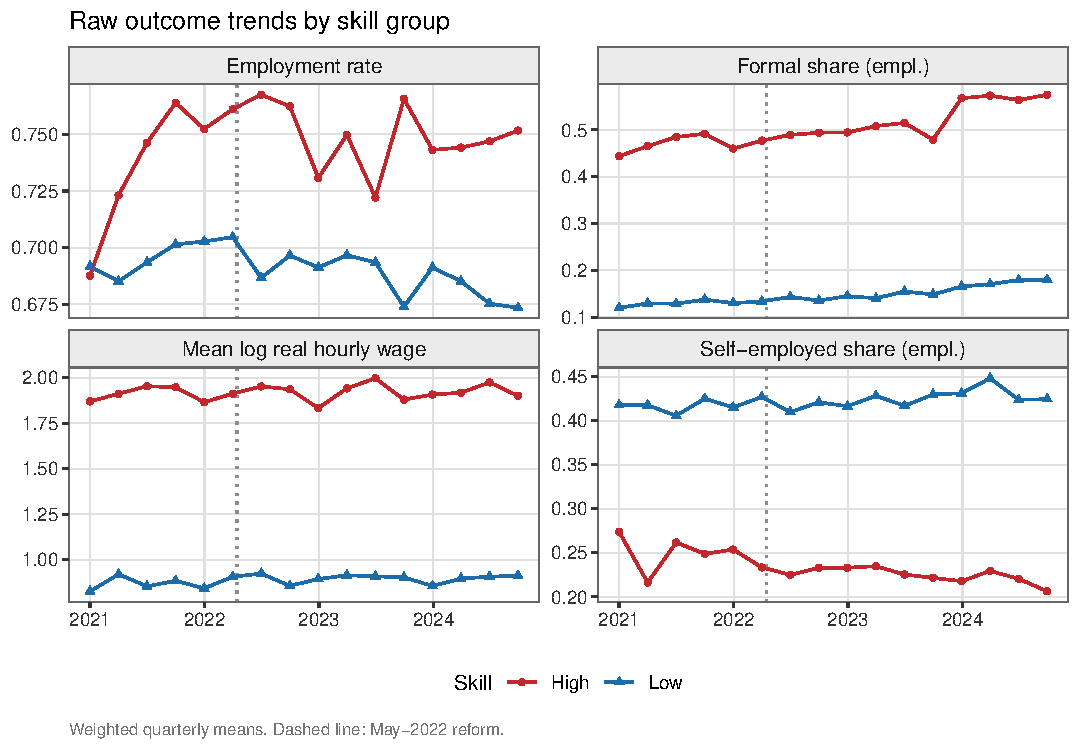
\includegraphics[width=0.95\textwidth]{fig2_raw_trends.pdf}
\caption{Raw outcome trends by skill group, 2021--2024. Weighted quarterly means for
low- and high-skilled workers. The dashed vertical line marks the May 2022 reform.}
\label{fig:trends}
\end{figure}

Figure~\ref{fig:bite} displays the regional variation in the bite of the minimum wage,
measured by the Kaitz index, the ratio of the new minimum to the pre-reform median
monthly-equivalent wage of private wage earners in each department. The index ranges
from about 0.79 in Ica to about 1.97 in Huánuco, and it exceeds one in eighteen of the
twenty-five departments, so that in much of the country the new minimum exceeds the
median wage. This variation is predetermined with respect to the reform and
provides the basis for the triple-difference and continuous-intensity checks in
Section~\ref{sec:robustness}.

\begin{figure}[!t]
\centering
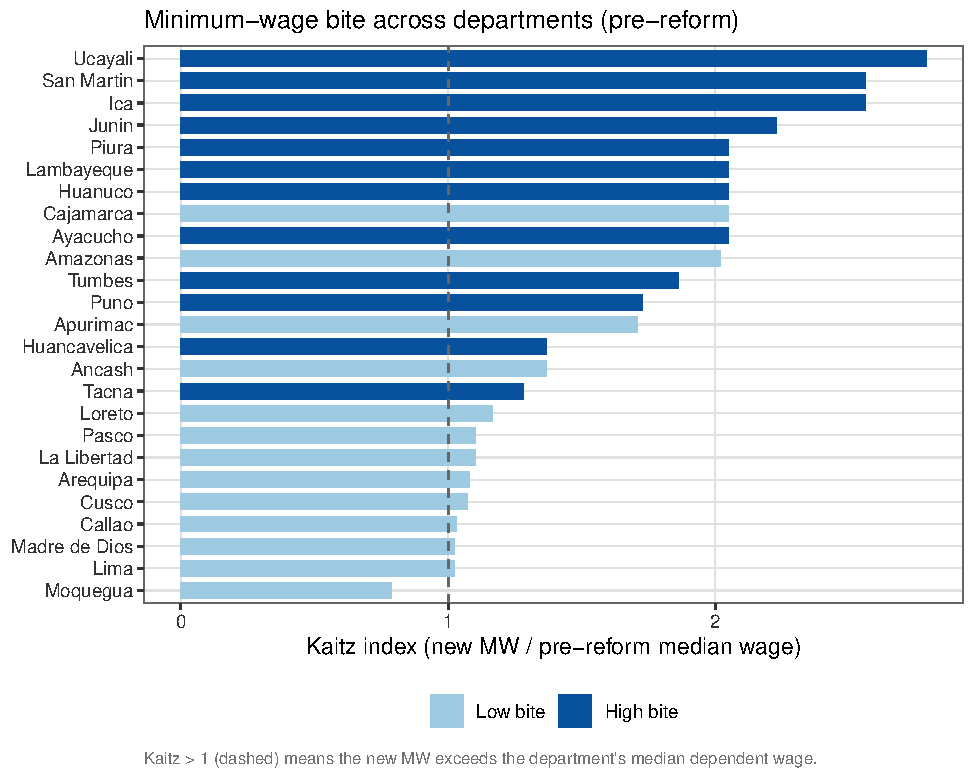
\includegraphics[width=0.72\textwidth]{fig3_regional_bite.pdf}
\caption{Regional variation in the bite of the minimum wage. The Kaitz index is the
ratio of the new minimum wage (1,025 soles) to the department's median monthly-equivalent
wage of private wage earners in the pre-reform quarters. Departments above the dashed
line have a median wage below the new minimum.}
\label{fig:bite}
\end{figure}

\section{Empirical strategy}\label{sec:strategy}

\subsection{Potential outcomes and the estimand}

Let $i$ index individuals, $g\in\{\Low,\mathrm{High}\}$ their skill group, and $t$ the
quarter. The reform becomes effective in the second quarter of 2022, which I denote
$t^{\ast}$; define the post-reform indicator $\Post_t=\mathbf{1}\{t\ge t^{\ast}\}$ and
the treatment indicator $\Low_i=\mathbf{1}\{g_i=\Low\}$. Following the potential-outcomes
framework, let $Y_{it}(1)$ and $Y_{it}(0)$ denote the outcome of individual $i$ in
quarter $t$ with and without the reform being in force. The parameter of interest is the
average effect of the reform on the low-skilled, relative to the counterfactual in which
they had experienced the same evolution as the high-skilled,
\begin{equation}
\mathrm{ATT} \;=\; \mathbb{E}\!\left[\,Y_{it}(1)-Y_{it}(0)\;\middle|\;\Low_i=1,\;t\ge t^{\ast}\right].
\end{equation}
The data are repeated cross-sections rather than a panel, so the object is identified from
comparisons of group means over time rather than from within-person changes.

Because Peru's minimum wage is national and changes on a single date, there is no variation
in treatment \emph{timing}; every worker is exposed to the same policy at the same moment.
Identification instead rests on variation in the \emph{intensity} of exposure across skill
groups. The design is therefore a canonical two-group difference-in-differences with many
periods, not a staggered-adoption design. This distinction matters for the choice of
estimator. The recent econometric literature has shown that the two-way fixed-effects
estimator can be badly biased when treatment timing is staggered and effects are
heterogeneous \citep{goodmanbacon_2021, dechaisemartin_2020, sun_abraham_2021,
callaway_santanna_2021}. With a common treatment date, however, these problems do not
arise: the two-way fixed-effects estimator and its event-study analog recover a convex,
properly weighted average of treatment effects \citep{roth_2023_trending,
baker_larcker_wang_2022}. I nonetheless report the doubly robust estimator of
\citet{santanna_zhao_2020} as a complementary building block.

\subsection{Estimating equations}

My baseline specification is the two-way fixed-effects difference-in-differences model
\begin{equation}
Y_{idt} \;=\; \beta\,(\Low_i\times\Post_t) \;+\; \gamma\,\Low_i \;+\; \lambda_t \;+\; \mu_d
\;+\; X_{it}'\theta \;+\; \varepsilon_{idt},
\label{eq:twfe}
\end{equation}
where $d$ denotes the department, $\lambda_t$ are quarter fixed effects, $\mu_d$ are
department fixed effects, and $X_{it}$ is a vector of controls comprising age, its square,
sex, an urban indicator, marital status, and years of education (which captures variation
in attainment within skill groups). The coefficient $\beta$ is the difference-in-differences
estimate. The quarter fixed effects absorb any shock common to both skill groups in a given
quarter, including aggregate inflation, so that estimates in logs are invariant to whether
wages are expressed in nominal or in nationally deflated real terms. Observations are
weighted by the survey weights, and standard errors are clustered by department.

To trace the dynamics of the effect and to test the identifying assumption, I estimate the
dynamic event-study specification
\begin{equation}
Y_{idt} \;=\; \sum_{k\neq -1}\beta_k\,\bigl(\Low_i\times\mathbf{1}\{t-t^{\ast}=k\}\bigr)
\;+\; \gamma\,\Low_i \;+\; \lambda_t \;+\; \mu_d \;+\; X_{it}'\theta \;+\; \varepsilon_{idt},
\label{eq:event}
\end{equation}
where $k$ indexes quarters relative to the reform and the quarter immediately before the
reform ($k=-1$, the first quarter of 2022) is the omitted reference. The coefficients
$\beta_k$ for $k<0$ measure differential pre-trends between the skill groups and provide a
direct test of parallel trends; the coefficients for $k\ge 0$ trace the path of the effect.

\subsection{Identifying assumptions and threats}

Identification of the ATT from equation~\eqref{eq:twfe} requires that, absent the reform, the
outcomes of low- and high-skilled workers would have followed parallel paths, conditional on
the controls and fixed effects. Three threats deserve attention.

First, \emph{differential trends}. Education is correlated with sector, region, and formality,
and the two skill groups could have been on diverging paths for reasons unrelated to the
minimum wage. I assess this directly through the pre-reform event-study coefficients and a
joint test of their equality to zero, and I probe robustness to department-specific linear
trends. Because my window opens in the depth of the pandemic recovery, when the employment of
low- and high-skilled workers rebounded at different rates, I pay particular attention to the
first quarter of 2021 and report specifications that drop it.

Second, \emph{sensitivity to residual violations}. Even when pre-trends are statistically flat,
they need not be exactly zero. I therefore report the sensitivity analysis of
\citet{rambachan_roth_2023}, which asks how large a post-reform violation of parallel trends,
relative to the largest violation observed before the reform, would be needed to overturn each
conclusion.

Third, \emph{spillovers and general equilibrium}. If the reform displaces low-skilled workers
into the informal sector, it may indirectly depress wages there, and if high-skilled workers are
imperfect substitutes their outcomes could also move, contaminating the comparison group. I
cannot rule this out, and I interpret the estimates as relative effects. The comparison group is not
entirely unexposed, since a minority of high-skilled workers also earn near the floor through
informal or own-account work; this imperfect exposure attenuates my estimates toward zero, so
the design understates rather than overstates the true effect on the fully exposed. I assess the
plausibility of the comparison by showing that the median high-skilled wage sits well above the
floor and that the high-skilled event-study path shows no break at the reform.

\subsection{Inference}

The treatment is assigned at a coarse level, the skill group, which raises the standard concern
that conventional standard errors overstate precision \citep{bertrand_2004}. I address this in
several complementary ways. My baseline clusters by department, which allows arbitrary
within-department correlation across individuals and quarters; I report an alternative that
clusters by department and skill group; and I apply the bias-reduced CR2 small-sample correction
of \citet{pustejovsky_tipton_2018} to department-level collapsed cells, where it is
computationally feasible. Because these corrections may still be optimistic with a two-group
design, I complement them with randomization inference at the department level, permuting the
regional bite of the minimum wage across departments to construct an exact null distribution for
the exposure-intensity design.

\section{Main results}\label{sec:results}

\subsection{The wage response}

The central result of the paper is that the 2022 reform did not raise the real wages of
low-skilled workers relative to high-skilled workers. Column (1) of
Table~\ref{tab:main} reports the two-way fixed-effects difference-in-differences
estimate from equation~\eqref{eq:twfe}. The coefficient on the interaction of the
low-skill indicator with the post-reform indicator is $-0.009$ for the log real hourly
wage, with a standard error of $0.022$, an estimate that is economically small and
statistically indistinguishable from zero. The implied point estimate is a relative
change of less than one percent, and the ninety-five percent confidence interval rules
out relative wage gains larger than about three percent. The result for log monthly
earnings is likewise a tight null. The doubly robust estimator of
\citet{santanna_zhao_2020} in column (2) is negative and imprecise but tells the same
qualitative story of no positive wage effect.

The dynamic event study confirms that this null is not an artifact of averaging over
offsetting periods. The top-left panel of Figure~\ref{fig:event} plots the coefficients
$\beta_k$ from equation~\eqref{eq:event} for the log real hourly wage. The pre-reform
coefficients are small and statistically insignificant, and a joint test of their
equality to zero does not reject, with a $p$-value of $0.60$ reported in column (3) of
Table~\ref{tab:main}. After the reform the coefficients hover around zero with no
discernible break. The wage distribution tells a consistent story:
Figure~\ref{fig:dist} shows the earnings distribution of low-skilled wage employees
before and after the reform, with the old and new minima marked. There is a visible mass
of workers near the old minimum, but the distribution does not shift appreciably toward
the new floor, and a large share of workers remain below it, reflecting the pervasive
non-compliance documented in Section~\ref{sec:data}.

\begin{table}[H]\centering
\caption{Difference-in-differences estimates of the 2022 minimum-wage reform}\label{tab:main}
\begin{threeparttable}
\begin{tabular}{lccc}
\toprule
Outcome & (1) TWFE DiD & (2) Doubly robust & (3) Pre-trend $p$ \\
\midrule
Log real hourly wage & -0.009 & -0.058 & 0.597 \\
 & (0.022) & (0.054) & \\
 & \multicolumn{2}{c}{\footnotesize $N=89,419$, $\bar{y}=1.361$} & \\
Log real monthly earnings & 0.005 & -0.034 & 0.038 \\
 & (0.019) & (0.054) & \\
 & \multicolumn{2}{c}{\footnotesize $N=91,937$, $\bar{y}=6.532$} & \\
Employment & -0.025$^{***}$ & 0.020 & 0.000 \\
 & (0.005) & (0.041) & \\
 & \multicolumn{2}{c}{\footnotesize $N=296,954$, $\bar{y}=0.708$} & \\
Labour force participation & -0.007 & -0.015 & -- \\
 & (0.005) & (0.036) & \\
 & \multicolumn{2}{c}{\footnotesize $N=296,954$, $\bar{y}=0.745$} & \\
Formal employment & -0.036$^{***}$ & 0.009 & 0.443 \\
 & (0.007) & (0.027) & \\
 & \multicolumn{2}{c}{\footnotesize $N=214,209$, $\bar{y}=0.270$} & \\
Self-employment & 0.029$^{***}$ & 0.053$^{**}$ & 0.000 \\
 & (0.006) & (0.024) & \\
 & \multicolumn{2}{c}{\footnotesize $N=214,209$, $\bar{y}=0.357$} & \\
Weekly hours & 0.810$^{***}$ & -0.453 & 0.109 \\
 & (0.182) & (1.041) & \\
 & \multicolumn{2}{c}{\footnotesize $N=210,534$, $\bar{y}=40.709$} & \\
Paid below the MW & -0.002 & 0.003 & 0.550 \\
 & (0.009) & (0.024) & \\
 & \multicolumn{2}{c}{\footnotesize $N=91,937$, $\bar{y}=0.496$} & \\
\bottomrule
\end{tabular}
\begin{tablenotes}\footnotesize
\item Notes: Each row is a separate regression. Column (1) reports the two-way fixed-effects DiD coefficient on $\mathrm{Low}\times\mathrm{Post}$ from equation~\eqref{eq:twfe}, with department and quarter fixed effects and controls (age, age squared, sex, urban, marital status, years of education). Column (2) reports the doubly robust DiD estimator of \citet{santanna_zhao_2020} collapsing to pre/post and dropping the transition quarter. Column (3) is the $p$-value of a joint test that the pre-reform event-study interactions are zero. Standard errors clustered by department in parentheses; all estimates are weighted by ENAHO survey weights. $^{*}p<0.1$, $^{**}p<0.05$, $^{***}p<0.01$.
\end{tablenotes}
\end{threeparttable}\end{table}


That the reform failed to lift wages at the bottom is not, in this setting, a surprising
result. The nominal increase of ten percent was substantially eroded by inflation of
about eight percent over 2022, so the real value of the floor rose only modestly. More
fundamentally, most low-skilled workers are informal or self-employed, for whom the
statutory minimum is not enforced. For them the minimum wage is at best a norm, and the
data suggest it did not operate as a binding one around this reform. The precise null
stands in contrast to the ``lighthouse'' pattern found for the 2016 reform by
\citet{jimenez_2023}, and we return to this contrast in Section~\ref{sec:discussion}.

\subsection{Employment and its composition}

If the reform did not raise pay, did it affect employment or its composition? Here the
evidence is more suggestive than conclusive, and it points to adjustment along the margin
between formal and informal work rather than to large changes in the level of employment.

The estimated effect on the probability of formal employment among the employed is
$-0.036$ (column 1 of Table~\ref{tab:main}), a decline of about three and a half
percentage points for low-skilled relative to high-skilled workers, and it is precisely
estimated under department clustering. The pre-trend test does not reject parallel trends
($p=0.44$), and the event study in Figure~\ref{fig:event} shows relative formality of the
low-skilled drifting down after the reform. Mirroring this, the probability of
self-employment rises by about three percentage points, an estimate that is statistically
significant and, as shown below, robust to randomization inference. Taken together these
two results describe a reallocation of low-skilled workers away from formal salaried jobs
and toward own-account work, the classic informalization margin emphasized by
\citet{jaramillo_lopez_2006} for Peru and by \citet{ham_2018_honduras} for Honduras. Weekly hours
in the main occupation rise modestly, consistent with a shift toward self-employment,
where hours are less constrained.

The effect on the overall employment rate is negative, at about $-2.5$ percentage points,
but it is the least robust of our estimates. As the event study makes clear, the employment
series carries a differential pre-trend concentrated in the first quarter of 2021, when the
labor market was still recovering unevenly from the pandemic across skill groups. Once that
quarter is excluded the pre-trend test no longer rejects, but the point estimate also
attenuates, and the effect does not survive our more conservative inference procedures. We
therefore treat the employment-level result as inconclusive and place little weight on it,
reserving the interpretive emphasis for the compositional shift, which is more stable.
Finally, the indicator for being paid below the minimum shows no significant change, meaning
that the reform did not measurably improve compliance at the bottom of the distribution.

\begin{figure}[H]
\centering
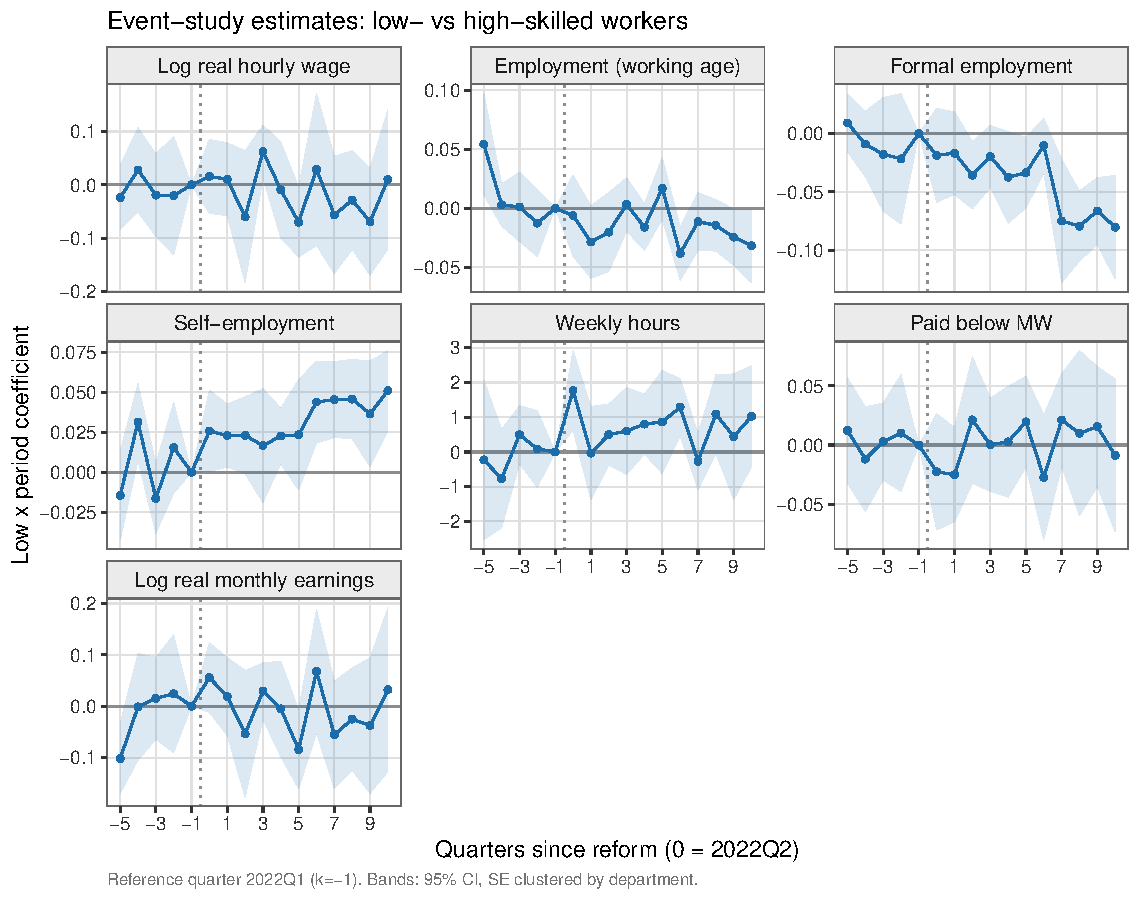
\includegraphics[width=0.98\textwidth]{fig5_event_study.pdf}
\caption{Event-study estimates of the 2022 reform. Each panel plots the coefficients
$\beta_k$ on the interaction of the low-skill indicator with quarter indicators from
equation~\eqref{eq:event}, relative to the omitted quarter 2022Q1 ($k=-1$). The reform is
effective at $k=0$ (2022Q2). Shaded bands are ninety-five percent confidence intervals with
standard errors clustered by department.}
\label{fig:event}
\end{figure}

\begin{figure}[H]
\centering
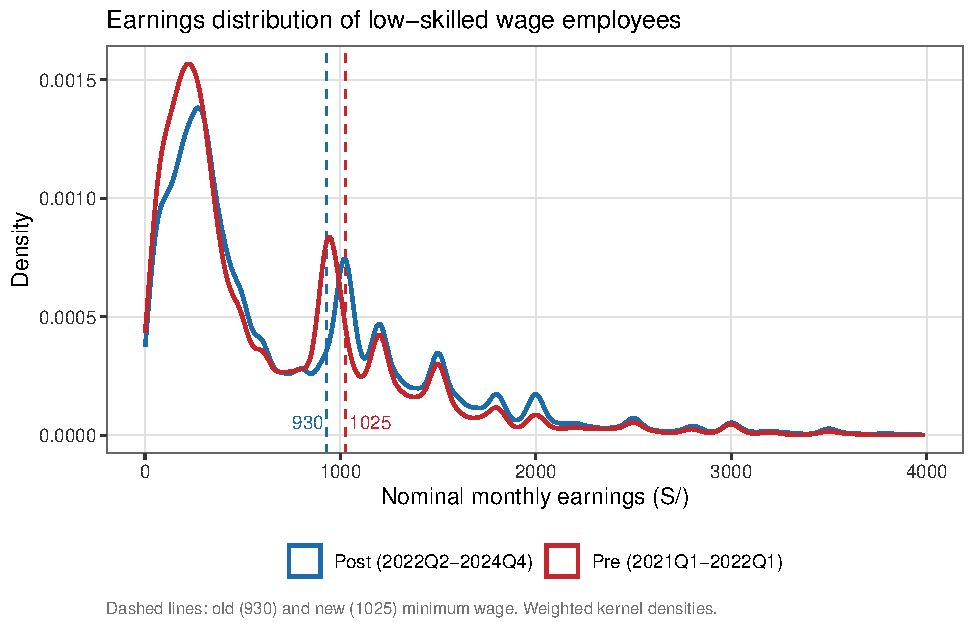
\includegraphics[width=0.72\textwidth]{fig4_wage_distribution.pdf}
\caption{Earnings distribution of low-skilled wage employees, before and after the reform.
Weighted kernel densities of nominal monthly earnings, with the old (930) and new (1,025)
minimum wage marked by dashed lines.}
\label{fig:dist}
\end{figure}

\section{Robustness and inference}\label{sec:robustness}

This section subjects the main results to a battery of specification, inference, and
design checks, and then to an out-of-sample replication. The overall message is that the
wage null is very robust, the compositional results are moderately robust, and the
employment-level result is fragile.

\subsection{Specification robustness}

Table~\ref{tab:robspec} reports the $\mathrm{Low}\times\mathrm{Post}$ coefficient for the
four headline outcomes under eight alternative specifications: dropping the controls,
dropping the pandemic quarter of early 2021, adding department-specific linear trends,
restricting to prime-age workers, using an alternative education cutoff that removes the
categories at the boundary between the two groups, adding one-digit occupation and
industry fixed effects, and clustering by department and skill. The wage estimate remains
a tight null across every specification. The formality and self-employment estimates are
stable in sign and magnitude throughout, moving within a narrow band. The employment
estimate, by contrast, attenuates noticeably when the pandemic quarter is dropped or when
department-specific trends are included, which reinforces our reluctance to interpret it
causally.

\begin{table}[!tbp]\centering
\caption{Specification robustness of the DiD estimates}\label{tab:robspec}
\begin{threeparttable}
\footnotesize
\setlength{\tabcolsep}{4pt}
\begin{tabular}{lcccc}
\toprule
Specification & Log hourly wage & Employment & Formal empl. & Self-employment \\
\midrule
Baseline & -0.021 & -0.025$^{***}$ & -0.046$^{***}$ & 0.036$^{***}$ \\
 & (0.012) & (0.006) & (0.007) & (0.006) \\
 & \footnotesize[69,534] & \footnotesize[278,064] & \footnotesize[181,317] & \footnotesize[181,317] \\
No controls & -0.008 & -0.021$^{***}$ & -0.042$^{***}$ & 0.042$^{***}$ \\
 & (0.012) & (0.006) & (0.007) & (0.006) \\
 & \footnotesize[69,534] & \footnotesize[278,064] & \footnotesize[181,317] & \footnotesize[181,317] \\
Drop 2021Q1 (pandemic) & -0.023$^{*}$ & -0.014$^{***}$ & -0.042$^{***}$ & 0.031$^{***}$ \\
 & (0.012) & (0.005) & (0.008) & (0.005) \\
 & \footnotesize[65,279] & \footnotesize[259,135] & \footnotesize[168,908] & \footnotesize[168,908] \\
Department linear trends & -0.022$^{*}$ & -0.017$^{***}$ & -0.040$^{***}$ & 0.034$^{***}$ \\
 & (0.012) & (0.006) & (0.007) & (0.006) \\
 & \footnotesize[69,534] & \footnotesize[278,064] & \footnotesize[181,317] & \footnotesize[181,317] \\
Prime age (25--55) & -0.030$^{*}$ & -0.023$^{***}$ & -0.042$^{***}$ & 0.029$^{***}$ \\
 & (0.015) & (0.004) & (0.008) & (0.007) \\
 & \footnotesize[46,021] & \footnotesize[161,115] & \footnotesize[119,540] & \footnotesize[119,540] \\
Alternative education cutoff & -0.015 & -0.039$^{***}$ & -0.065$^{***}$ & 0.050$^{***}$ \\
 & (0.012) & (0.007) & (0.006) & (0.007) \\
 & \footnotesize[40,526] & \footnotesize[186,263] & \footnotesize[117,174] & \footnotesize[117,174] \\
Occupation \& industry FE & -0.007 & -0.016$^{***}$ & -0.036$^{***}$ & 0.027$^{***}$ \\
 & (0.011) & (0.003) & (0.006) & (0.005) \\
 & \footnotesize[69,534] & \footnotesize[213,810] & \footnotesize[181,317] & \footnotesize[181,317] \\
Cluster dept.$\times$skill & -0.021 & -0.025 & -0.046$^{***}$ & 0.036$^{***}$ \\
 & (0.013) & (0.020) & (0.007) & (0.007) \\
 & \footnotesize[69,534] & \footnotesize[278,064] & \footnotesize[181,317] & \footnotesize[181,317] \\
Low-skilled group linear trend & -0.021 & -0.005 & -0.004 & 0.006 \\
 & (0.019) & (0.008) & (0.010) & (0.009) \\
 & \footnotesize[69,534] & \footnotesize[278,064] & \footnotesize[181,317] & \footnotesize[181,317] \\
Include transition quarter (2022Q2) & -0.018 & -0.025$^{***}$ & -0.044$^{***}$ & 0.035$^{***}$ \\
 & (0.012) & (0.005) & (0.007) & (0.006) \\
 & \footnotesize[74,310] & \footnotesize[296,954] & \footnotesize[193,762] & \footnotesize[193,762] \\
Exclude agriculture (agrarian regime) & -0.022$^{*}$ & -- & -0.038$^{***}$ & 0.028$^{***}$ \\
 & (0.012) &  & (0.007) & (0.005) \\
 & \footnotesize[53,755] & \footnotesize[--] & \footnotesize[114,212] & \footnotesize[114,212] \\
Include public-sector workers & -0.002 & -- & -0.037$^{***}$ & 0.030$^{***}$ \\
 & (0.010) &  & (0.008) & (0.006) \\
 & \footnotesize[87,033] & \footnotesize[--] & \footnotesize[200,383] & \footnotesize[200,383] \\
\bottomrule
\end{tabular}
\begin{tablenotes}\footnotesize
\item Notes: Each cell is the $\mathrm{Low}\times\mathrm{Post}$ DiD coefficient (standard error clustered by department below; sample size in brackets) for the outcome in the column heading, under the specification in the row; all estimates are weighted by ENAHO survey weights, and Log hourly wage denotes the log real hourly wage. The baseline is equation~\eqref{eq:twfe}, which excludes the partially treated 2022Q2. The alternative education cutoff defines low-skilled as at most incomplete secondary and high-skilled as at least complete non-university tertiary, dropping the boundary categories. The agriculture exclusion and the public-sector inclusion apply to job-conditional outcomes only (industry and sector are undefined for non-workers). $^{*}p<0.1$, $^{**}p<0.05$, $^{***}p<0.01$.
\end{tablenotes}
\end{threeparttable}\end{table}


\subsection{Inference}

Because the treatment is assigned at the level of the skill group, we assess whether the
significance of the compositional results survives more demanding inference.
Table~\ref{tab:inference} collects the evidence. Columns (1) through (4) report
$p$-values for the baseline effect under department clustering, department-by-skill
clustering, the CR2 small-sample correction of \citet{pustejovsky_tipton_2018} applied to
department-level collapsed cells, and randomization inference that permutes the regional
bite of the minimum wage across departments. The self-employment effect is the most
resilient: it remains significant under department-by-skill clustering and under
randomization inference. The formality effect is significant under both clustering schemes
but only marginal under the most conservative CR2 and randomization procedures, which are
low-powered with twenty-five departments. The employment effect loses significance under
every procedure beyond simple department clustering. The wage null is, of course,
unaffected.

\begin{table}[!tbp]\centering
\caption{Inference robustness, design robustness, and out-of-sample validation}\label{tab:inference}
\begin{threeparttable}
\footnotesize
\begin{tabular}{lcccccc}
\toprule
Outcome & (1) Dept. & (2) Dept.$\times$skill & (3) CR2 & (4) RI (continuous) & (5) Continuous & (6) 2025 reform \\
\midrule
Log hourly wage & 0.106 & 0.126 & 0.854 & 0.029 & 0.017 & 0.002 \\
 & & & & & (0.012) & (0.011) \\
Employment & 0.000 & 0.210 & 0.507 & 0.003 & -0.034$^{***}$ & -0.002 \\
 & & & & & (0.012) & (0.005) \\
Formal empl. & 0.000 & 0.000 & 0.244 & 0.000 & -0.018$^{***}$ & -0.001 \\
 & & & & & (0.003) & (0.008) \\
Self-employment & 0.000 & 0.000 & 0.093 & 0.024 & 0.010$^{**}$ & -0.014$^{**}$ \\
 & & & & & (0.004) & (0.006) \\
\bottomrule
\end{tabular}
\begin{tablenotes}\footnotesize
\item Notes: Columns (1)--(3) report $p$-values for the baseline $\mathrm{Low}\times\mathrm{Post}$ effect under, respectively, department clustering (25 clusters), department$\times$skill clustering (50 clusters), and the CR2 small-sample correction \citep{pustejovsky_tipton_2018} applied to department-level collapsed cells. Column (4) reports the randomization-inference $p$-value for the CONTINUOUS-exposure design of column (5), not for the two-group $\mathrm{Low}\times\mathrm{Post}$ contrast, obtained by permuting the 25 regional Kaitz indices across departments (2{,}000 draws). Column (5) reports the continuous-exposure estimate, the coefficient on $\mathrm{Post}\times$(standardized department Kaitz index), with department-clustered standard errors in parentheses. Column (6) reports the $\mathrm{Low}\times\mathrm{Post}$ DiD estimate for the January-2025 reform (window 2024--2025), with department-clustered standard errors in parentheses. Log hourly wage denotes the log real hourly wage; all estimates are weighted by ENAHO survey weights. $^{*}p<0.1$, $^{**}p<0.05$, $^{***}p<0.01$.
\end{tablenotes}
\end{threeparttable}\end{table}


\subsection{Design robustness: bite intensity and triple differences}

Our identification rests on differential exposure by education, but the minimum wage also
bites differentially across regions, and this provides an independent source of variation.
Column (5) of Table~\ref{tab:inference} reports a continuous-exposure specification in the
spirit of \citet{card_1992}, which replaces the binary treatment with the standardized
department Kaitz index interacted with the post indicator. The results corroborate the
skill-based design: in departments where the minimum wage bites harder, formal employment
falls and self-employment rises by significantly more after the reform, while wages do not
respond. A triple-difference specification that interacts the skill contrast with an
indicator for high-bite departments is not statistically significant, which we read as a
lack of power in the binary regional split rather than as evidence against the mechanism,
given that the continuous version is informative.

\subsection{Sensitivity to violations of parallel trends}

Even flat pre-trends are estimated with error, so we apply the sensitivity analysis of
\citet{rambachan_roth_2023}. Figure~\ref{fig:honest} plots the robust confidence set for
the average post-reform effect on employment and formality as we allow the post-reform
violation of parallel trends to be as large as a multiple $\bar{M}$ of the largest
pre-reform violation. The formality effect remains bounded away from zero only for small
departures, up to about $\bar{M}=0.1$, and the self-employment effect only under near-exact
parallel trends, whereas the employment effect includes zero even under the smallest departure.
The compositional results are thus robust to conventional inference but sensitive to modest
trend violations, which reinforces our decision to emphasize the wage null, the one result
that is both precisely estimated and replicated out of sample.

\begin{figure}[H]
\centering
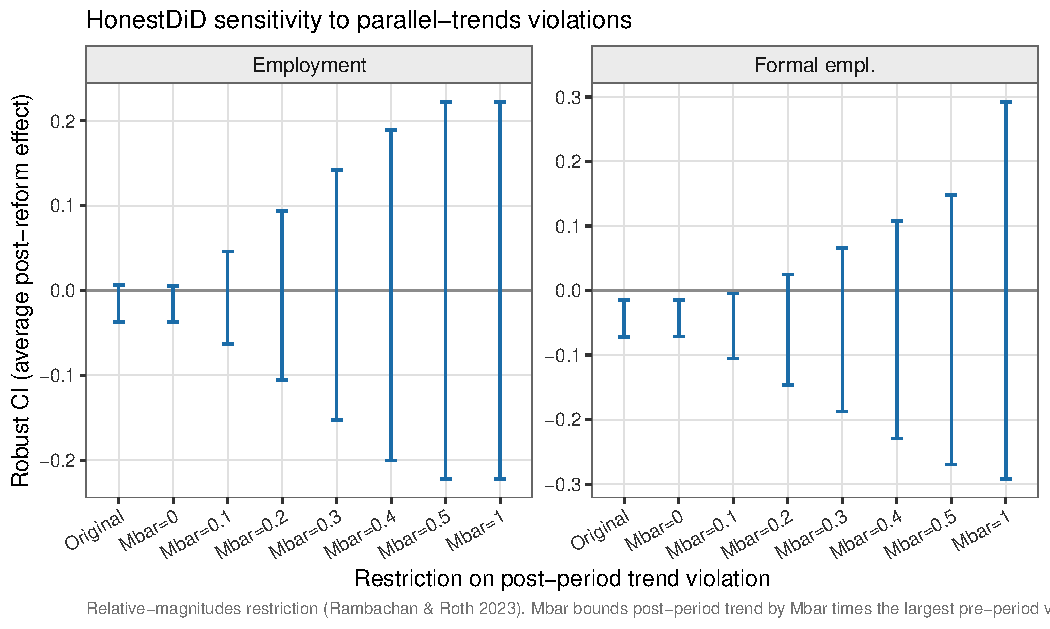
\includegraphics[width=0.8\textwidth]{fig7_honestdid.pdf}
\caption{Sensitivity to violations of parallel trends
\citep{rambachan_roth_2023}. Robust confidence sets for the average post-reform effect
under the relative-magnitudes restriction, which bounds the post-reform trend violation by
$\bar{M}$ times the largest pre-reform violation.}
\label{fig:honest}
\end{figure}

\subsection{Placebo reforms and leave-one-out}

We assign fake reforms to each interior quarter of the pre-reform window and re-estimate
the DiD using only pre-reform data. The wage placebos are uniformly null, the formality and
self-employment placebos are mostly null with one marginal case, but the employment placebos
are significant, which is a direct symptom of the pandemic-driven pre-trend in that outcome.
Leave-one-department-out and leave-one-quarter-out re-estimation leave the point estimates
essentially unchanged for all four outcomes, indicating that no single region or quarter
drives the results. These checks are reported in the appendix.

\subsection{Out-of-sample validation: the 2025 reform}

Finally, we replicate the entire design around the second reform, which raised the minimum
wage to 1,130 soles on 1 January 2025, using the 2024 and 2025 quarters. This reform is of
almost identical magnitude to the 2022 one but occurs in a calmer, post-pandemic
environment. Column (6) of Table~\ref{tab:inference} reports the estimates. The wage effect
is again a null, which strengthens our central finding considerably: across two independent
reforms in different macroeconomic conditions, the minimum wage did not raise the relative
wages of low-skilled workers. The compositional effects, however, do not replicate: the
formality and employment effects are null around the 2025 reform, and the self-employment
effect reverses sign. We take this seriously. It implies that the reallocation we document
around 2022 is specific to that episode and may reflect the unusual dynamics of the
post-pandemic labor market rather than a stable structural response to the minimum wage. The
one conclusion that survives out of sample is the wage null.

\section{Heterogeneity and distributional effects}\label{sec:heterogeneity}

\subsection{Who adjusts?}

Figure~\ref{fig:het} reports the low- versus high-skilled DiD estimate for each headline
outcome within demographic and regional subgroups.\footnote{Each estimate is the
within-subgroup difference-in-differences, so it asks whether the low- versus high-skilled
contrast differs across, say, men and women, not the level effect for a subgroup.} Three
patterns stand out and are
consistent with economic intuition about where the minimum wage binds hardest.

First, no subgroup shows wage gains. Whether defined by sex, age, area, or regional bite,
every subgroup wage estimate is negative or indistinguishable from zero. The absence of a
pay response is a pervasive feature of the data rather than an average that masks
offsetting effects.

Second, the compositional adjustment scales with exposure. The decline in formal
employment is larger in high-bite departments ($-5.5$ percentage points) than in low-bite
departments ($-3.6$ points), and the rise in self-employment likewise ($+5.0$ against
$+2.8$ points). This dose-response pattern is what a causal effect of the wage floor
should produce, and it is the cross-sectional counterpart of the continuous-exposure
results in Section~\ref{sec:robustness}. The employment-level estimate, by contrast, does
\emph{not} scale with the bite (it is smaller and insignificant in high-bite
departments), which is further reason to attribute it to differential recovery rather
than to the reform.

Third, the reallocation is concentrated among the young and among women. The decline in
formal employment is largest for workers aged fourteen to twenty-five ($-5.8$ points) and
for women ($-5.5$ points), the groups whose wages are most likely to sit near the floor
and whose attachment to formal employment is most tenuous; the rise in self-employment is
twice as large for women as for men. For workers over forty-five the formality effect is
near zero, though their self-employment also rises. This mirrors the emphasis on youth in
the earlier Peruvian literature \citep{cespedes_2005, jaramillo_lopez_2006} and the
emphasis on women and the least skilled in the developing-country evidence
\citep{katzkowicz_2021_uruguay, lemos_2009}.

\begin{figure}[!t]
\centering
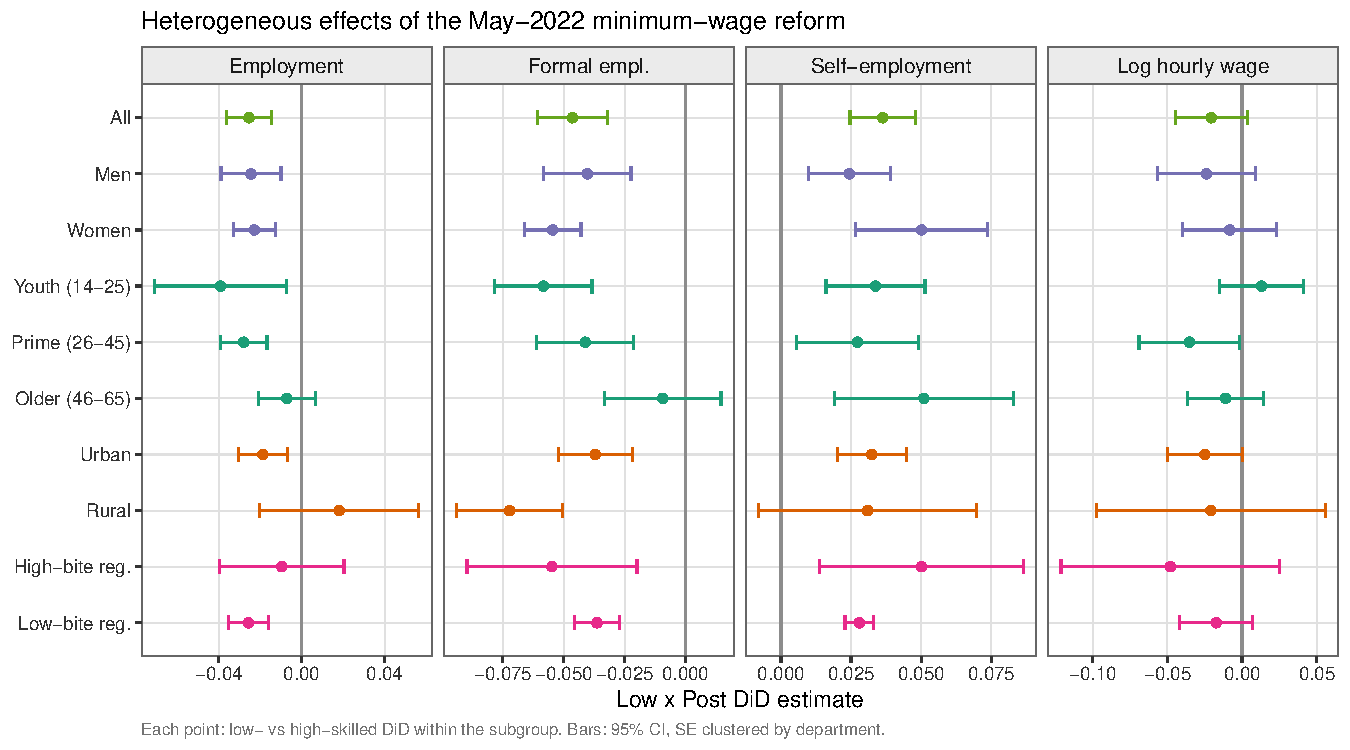
\includegraphics[width=0.98\textwidth]{fig6_heterogeneity.pdf}
\caption{Heterogeneous effects of the 2022 reform. Each point is the
$\mathrm{Low}\times\mathrm{Post}$ DiD estimate within the indicated subgroup, with
ninety-five percent confidence intervals based on standard errors clustered by department.}
\label{fig:het}
\end{figure}

\subsection{Adjustment margins}

Where exactly does the reallocation happen? Four mechanism-oriented margins sharpen
the picture (Appendix Table~\ref{tab:margins}). First, the share of low-education
wage earners employed \emph{without a written contract} rises by 3.1 percentage
points relative to high-education wage earners, so informalization operates within
wage employment and not only through exits into self-employment.\footnote{The
contract item was dropped from the reduced questionnaire applied in fifteen regions
in February 2021; I code those observations as missing rather than as lacking a
contract, which matters for this margin.} Second, employment
recomposes toward \emph{micro units}: the probability that a low-education worker is
employed in an establishment of at most twenty workers rises by 2.8 points, and small
units are precisely where enforcement is thinnest. Third, using INEI's decomposition
of informal employment (available through 2023), the displaced margin lands in the
\emph{informal sector} proper (+2.4 points) rather than in unregistered jobs inside
formal firms (+0.8, insignificant): workers did not stay with formal employers under
the table; they moved to informal productive units. Fourth, the share of wage
earners with under a year of tenure does not move, so the adjustment is not visible
as a hiring freeze among those who remain wage earners.

Two further subgroup splits locate the burden. The compositional effects are
concentrated almost entirely among \emph{non-heads} of household (secondary
earners, whose formality falls 6.8 points against a null for household heads) and
among non-indigenous workers, consistent with the urban coastal labor markets where
formal employment at the floor is concentrated. The marginal formal jobs that
dissolved were, in short, those of secondary earners in small urban firms.

\subsection{Distributional wage effects}

The absence of an average wage effect could in principle conceal offsetting movements at
different points of the wage distribution, since a minimum wage is expected to compress the
lower tail. To examine this I estimate unconditional quantile (recentered influence
function) regressions in the manner of \citet{firpo_fortin_lemieux_2009}, applying the DiD
specification to the influence function of each decile of the log real hourly wage.
Figure~\ref{fig:rif} plots the $\mathrm{Low}\times\mathrm{Post}$ coefficient across
deciles. The estimates are non-positive at every decile, mostly between $-2$ and $-4$
percent and significant at a few middle deciles; crucially, there is no positive effect at
the lower deciles, where a binding and enforced minimum wage would compress the
distribution from below. The distributional evidence therefore reinforces the absence of
a pay response: the reform did not lift the lower tail of the low-skilled wage
distribution relative to the high-skilled. This is consistent with the earnings
distribution in Figure~\ref{fig:dist}, which shows little movement toward the new floor,
and with the interpretation that in a labor market with widespread non-compliance the
statutory minimum did not bind for most low-skilled workers.

\begin{figure}[!t]
\centering
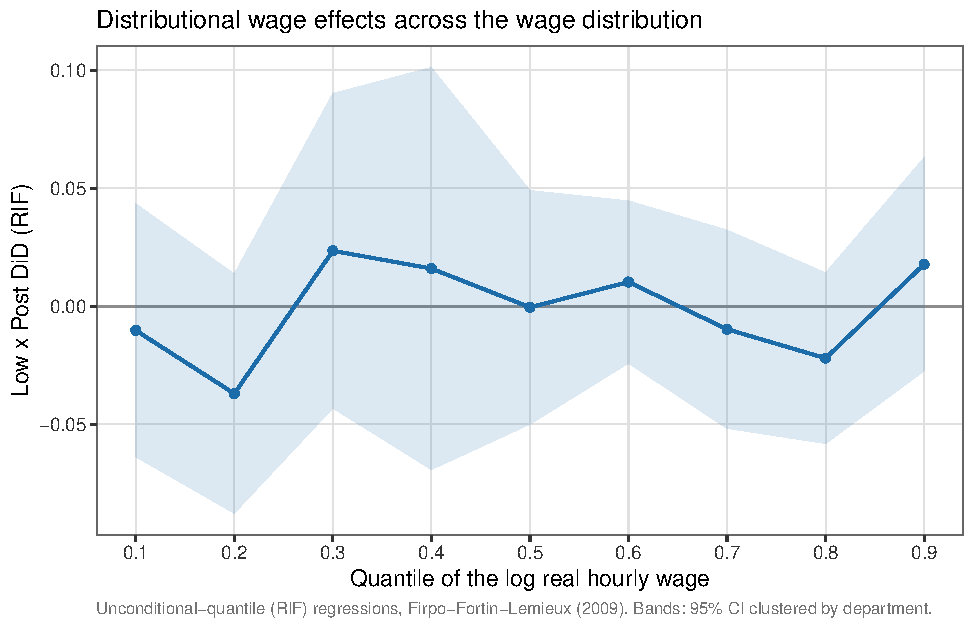
\includegraphics[width=0.72\textwidth]{fig8_rif_quantile.pdf}
\caption{Distributional wage effects. Each point is the $\mathrm{Low}\times\mathrm{Post}$
DiD coefficient from an unconditional-quantile (RIF) regression at the indicated decile of
the log real hourly wage \citep{firpo_fortin_lemieux_2009}. Bands are ninety-five percent
confidence intervals clustered by department.}
\label{fig:rif}
\end{figure}

\section{Discussion}\label{sec:discussion}

\subsection{Mechanisms}

The evidence describes a minimum wage with little purchase on the pay of the workers it is
meant to protect. The wage null is my most robust result: it holds across two reforms, across
the wage distribution, and across demographic groups. Two features of the institutional
environment make it intelligible. The first is inflation. The 2022 increase of ten percent in
nominal terms met consumer price inflation of roughly eight percent, so the real value of the
floor barely rose and then eroded. The second, and more fundamental, is informality. Most
low-skilled Peruvian workers are informal or self-employed, and for them the statutory minimum
is not enforced; compliance is high only within registered formal firms, which employ a
minority of the low-skilled. A floor that reaches only a small and selected part of the
relevant labor force cannot move its average wage by much, and the earnings distribution in
Figure~\ref{fig:dist} confirms that it did not.

If the reform did not raise pay, did it move anything else? Around 2022 I find a shift from
formal employment toward self-employment, concentrated among the young and among women. The
natural mechanism is the classic one, a binding floor in the covered sector inducing some
reallocation to the uncovered sector, the displacement channel that \citet{jaramillo_lopez_2006}
documents for Peru and \citet{ham_2018_honduras} for Honduras; the accompanying rise in hours
is consistent with movement toward self-employment, where hours are less constrained. I read
this cautiously, because the compositional effect does not survive my most demanding inference
and does not reappear around the 2025 reform. Its reversal out of sample suggests that part of
what I capture around 2022 reflects the uneven post-pandemic recovery rather than a structural
response to the minimum wage, so I present the reallocation as a feature of the 2022 episode
rather than as a general law.

\subsection{Reconciliation with the previous literature}

My results sit comfortably with some of the prior evidence and in tension with the rest, and
the pattern is itself informative. They echo the older Peruvian work of
\citet{jaramillo_lopez_2006}, who found the 2003 reform largely innocuous with displacement
toward informality, and of \citet{cespedes_2005}, who found effects concentrated among the
young. They are consistent with the broad international finding that minimum wage increases in
this range produce small employment effects \citep{card_krueger_1995, cengiz_2019}.

The tension is with the most recent Peruvian study. \citet{jimenez_2023} finds that the 2016
reform raised formal wages by four to five percent and increased formality, a lighthouse
pattern that I do not reproduce for 2022. Three differences plausibly account for the
divergence. The 2016 increase occurred in a low-inflation period, so its real bite was larger
and more durable than that of the inflation-eroded 2022 increase. The identification differs:
\citet{jimenez_2023} uses a department-level dose defined on the formal wage distribution,
while I contrast low- and high-education workers at the individual level, a design that places
more weight on the large informal segment of the low-skilled. And the macroeconomic setting
differs, stable growth in 2016 against a post-pandemic recovery in 2022. Taken together, these
suggest that the labor-market effects of the Peruvian minimum wage are state-dependent, closer
to the lighthouse pattern when the real increase is substantial and the economy is stable, and
muted when inflation erodes the increase and informality absorbs the adjustment.

\subsection{External validity and limitations}

Four limitations bound the interpretation. First, identification rests on the assumption that,
absent the reform, low- and high-education workers would have followed parallel paths. I test
this where possible and bound the consequences of its failure, but I cannot rule out
differential shocks correlated with education in the volatile 2021--2022 window; this is why I
lean on the wage result, whose pre-trends are flat and which replicates out of sample, and
treat the employment-level result as inconclusive. Second, the design identifies effects on
low-skilled workers relative to high-skilled workers. If the reform also reached the
high-skilled, through general-equilibrium spillovers or ripple effects up the distribution, my
estimates mismeasure the absolute effect on the low-skilled; I judge large spillovers to the
tertiary-educated unlikely given that their median wage sits well above the floor, and I note
that because the comparison group is not entirely unexposed, any resulting bias attenuates my
estimates toward zero, so the wage null is a conservative reading. Third, the data are repeated
cross-sections, so I cannot follow individuals across the reform or separate changes in the
composition of the employed from changes in individual outcomes. Fourth, informality in 2024
is measured with a reconstructed indicator rather than the official one; my robustness checks
suggest this does not drive the results, but it adds measurement error. Finally, the window
spans at most eleven post-reform quarters, so I speak to short- and medium-run effects and not
to the long-run adjustment of capital or firm entry and exit.

\subsection{Policy implications}

The results carry a sober message for minimum wage policy in a high-informality economy. A
floor that goes unenforced for most of its intended beneficiaries does little to raise their
pay, and where it does bind, in the formal sector, it may nudge some workers toward less
protected arrangements. Raising the minimum wage is therefore an imperfect instrument for
lifting the earnings of the low-skilled in Peru, a conclusion that echoes
\citet{jaramillo_lopez_2006}. This is not to say the minimum wage is harmless or useless; my
estimates are relative and my window is short. But it does imply that formalization and
enforcement are preconditions for the floor to reach the workers it is designed to protect.
Absent them, the margin of adjustment is the composition of employment rather than the level of
pay.

\section{Conclusion}\label{sec:conclusion}

I have studied how Peru's 2022 minimum wage increase, from 930 to 1,025 soles, affected
workers with different levels of education, using sixteen quarters of the ENAHO employment
survey and a difference-in-differences design that exploits the sharply different exposure
of low- and high-education workers to a single national reform. My central finding is a
precisely estimated null: the reform did not raise the real wages of low-education workers
relative to high-education workers, at the mean or anywhere in the distribution. This
conclusion is robust to a wide range of specifications and, importantly, replicates around
the subsequent reform of January 2025. Around the 2022 reform I also find evidence of a
shift from formal employment toward self-employment, concentrated among the young and among
women, though this compositional effect is less robust and does not carry over to the 2025
episode. The overall employment effect cannot be pinned down and is confounded by the
uneven post-pandemic recovery.

The most economical reading of these results is that, in a labor market where informality is
pervasive and enforcement is weak, a moderate and inflation-eroded increase in the statutory
minimum does little to lift the pay of the low-skilled and instead operates, when it
operates at all, on the margin between formal and informal work. This qualifies the
lighthouse view of the Peruvian minimum wage that emerges from studies of earlier reforms
and points to the informal margin as the central channel of adjustment.

Two directions for future research follow. The first is to exploit the panel component of
ENAHO, where available, to follow individuals across reforms and to distinguish
compositional from individual-level effects. The second is to study the interaction between
minimum wage policy and formalization policy directly, since my results suggest that the
returns to raising the floor depend on whether the floor can be made to bind. As additional
post-reform quarters accumulate, it will also become possible to trace the longer-run
adjustment that a short window such as mine cannot capture.


\section*{Declarations}
\noindent\textbf{Declarations of interest:} none.\\
\textbf{Funding:} this research received no specific grant from any funding agency in the
public, commercial, or not-for-profit sectors.\\
\textbf{Data availability:} the ENAHO microdata are publicly available from the Instituto
Nacional de Estadística e Informática (INEI). The code that reproduces every table and
figure is available in the online replication repository.

\newpage
\bibliography{references}

\newpage
\appendix
\section{Data appendix}\label{app:data}

\subsection{Sample and variable construction}

I pool the twenty quarterly ENAHO employment modules (module 500) for 2021Q1--2025Q4;
the main analysis uses 2021Q1--2024Q4 and the validation uses 2024Q1--2025Q4. The
working-age sample comprises individuals aged 14 to 65 with non-missing education. All
statistics use the module employment weight (\texttt{fac500a}). This weight is
calibrated so that the full year of interviews expands to the annual population
projection; each quarterly subsample therefore expands to roughly one fourth of the
population, which is immaterial for the weighted means, shares, and regression
estimates used throughout (numerator and denominator scale together) and would matter
only for population totals, which I never estimate. The quarterly partition follows
the interview month and matches the survey's own design: quarterly national inference
is an official inference level of ENAHO in the technical sheets of both 2021 and 2025,
and the non-panel sample revisits the same conglomerates in the same months every
year. I verify both properties in the microdata for the full window: all 5{,}359
conglomerates appear in every year from 2021 to 2025, the overlap of primary sampling
units between the same quarter of consecutive years ranges from 70 to 92 percent
(against 2 to 5 percent between different quarters), and each quarter is an
internally balanced replica of the design. Two survey changes over the window are
worth recording. First, the mixed interview modality adopted during the pandemic
(face-to-face prioritized, telephone follow-up for absent members) remained the
standard through 2025, so the mode is broadly consistent across my study period; the
one exception is February 2021, when a reduced telephone questionnaire in fifteen
regions dropped, among other items, the contract-type question (missing for half of
that month's wage earners), which affects none of the baseline outcomes (2021
informality comes from INEI's official indicator and income items were retained) and
is handled explicitly in the one appendix margin that uses contracts. Second, the
2025 technical sheet describes the design as two-stage with urban conglomerates of
about 140 dwellings, against the multi-stage description of 2021; the conglomerate
identifiers and counts are nonetheless continuous across the window, so this is a
reframing of the documentation rather than a break in the sample. Departments are the 25
first-level administrative units derived from the first two digits of \texttt{ubigeo};
the urban indicator is derived from the sampling stratum.

\paragraph{Education and skill groups.} Educational attainment is ENAHO variable
\texttt{p301a}. I verified its coding against the weighted attainment distribution.
Low-skilled workers are those with \texttt{p301a} in 1--6 (no education through complete
secondary); high-skilled workers are those with \texttt{p301a} in 7--11 (non-university
higher through postgraduate). Special education (code 12) and missing values are excluded.

\paragraph{Labor income and wages.} ENAHO records the pay of wage earners per pay period:
\texttt{p524a1} is the gross payment including overtime and \texttt{p523} its frequency
(daily, weekly, fortnightly, or monthly). Fifty-four percent of low-education wage
earners are paid at non-monthly frequencies, against fifteen percent of high-education
wage earners, so I convert all payments to monthly equivalents using the same factors
implied by INEI's own annualized income variable (\texttt{i524a1}): 25 for daily, $52/12$
for weekly, 2 for fortnightly, and 1 for monthly. Wage earners comprise employees and
domestic workers (\texttt{p507} in $\{3,4,6\}$); domestic workers have been entitled to
the minimum wage since Law 31047. For employers and own-account workers, labor income is
net profit (\texttt{p530a}), which is already monthly. Because reported income refers to
the month before the interview, I deflate at that reference month (January interviews
roll back to December of the previous year) using the Lima consumer price index
rebased to December 2021, and I evaluate the statutory minimum in force in the same
reference month when classifying workers as paid below the floor. The real hourly wage
divides monthly-equivalent labor income by $4.345$ times weekly hours in the main
occupation (\texttt{p513t}, imputed where missing). Wage outcomes exclude public-sector
workers, whose pay is set by separate scales, and are winsorized once at the 0.5th and
99.5th percentiles of the pooled private wage-earner sample.

\paragraph{Informality.} INEI's official informal-employment indicator (\texttt{ocupinf},
coded 1 for informal and 2 for formal in these files) is present for 2021--2023 but absent
for 2024--2025. I reconstruct a consistent indicator from primitives available in every
year. A wage employee or domestic worker is classified as formal if affiliated to a
pension system (\texttt{p558a1}--\texttt{p558a4}, whose selected options are marked with
their option codes rather than with ones) or holding a formal labor contract
(\texttt{p511a} in 1--6); an employer or own-account worker is classified as formal if the
productive unit is registered (\texttt{p510a1}); unpaid family workers are always informal.
Validated against \texttt{ocupinf} on the overlapping years 2021--2023, this rule agrees
with the official classification for 87.8 percent of employed workers and yields an
informality rate of 74.9 percent against the official 79.1 percent. I use the official
indicator wherever available and the reconstruction only for 2024--2025; within the
2024--2025 validation window the indicator is reconstructed in every quarter, so it is
measured consistently there.

\paragraph{Minimum wage and bite.} The statutory minimum wage schedule is taken from the
decrees and verified against the Banco Central de Reserva del Perú series (PN02124PM);
the CPI deflator is BCRP series PN38705PM (Lima, December 2021 $=$ 100), and both inputs
are regenerated by a documented script in the replication package. The department Kaitz
index is the ratio of the post-reform minimum (1,025 soles) to the department's
pre-reform (2021Q1--2022Q1) weighted median monthly-equivalent wage of private wage
earners. The fraction-affected measure is the pre-reform weighted share of private wage
earners paid below 1,025 soles.

\subsection{Supplementary results}

Table~\ref{tab:ddd} reports the triple-difference estimates and Table~\ref{tab:loo}
the leave-one-out stability ranges discussed in Section~\ref{sec:robustness};
Tables~\ref{tab:expocells}--\ref{tab:margins} collect the exposure-design diagnostics,
the sectoral and occupational checks, the selection bounds and power calculations, the
synthetic-DiD and pre-test-power results, and the adjustment margins.
Table~\ref{tab:placebo} reports the in-time placebo reforms and confirms that the wage
placebos are null while the employment placebos are contaminated by the pandemic
pre-trend. The doubly robust estimates of \citet{santanna_zhao_2020} appear alongside
the two-way fixed-effects estimates in Table~\ref{tab:main}.
Figure~\ref{fig:val2025} shows the event study around the January-2025 reform used in
the out-of-sample validation.

\begin{table}[H]\centering
\caption{Triple-difference estimates: $\mathrm{Low}\times\mathrm{Post}\times\mathrm{HighBite}$}\label{tab:ddd}
\begin{threeparttable}
\begin{tabular}{lc}
\toprule
Outcome & DDD estimate \\
\midrule
Log hourly wage & -0.027 \\
 & (0.038) \\
Employment & 0.015 \\
 & (0.016) \\
Formal empl. & -0.018 \\
 & (0.018) \\
Self-employment & 0.026 \\
 & (0.018) \\
\bottomrule
\end{tabular}
\begin{tablenotes}\footnotesize
\item Notes: Coefficient on the triple interaction $\mathrm{Low}\times\mathrm{Post}\times\mathrm{HighBite}$, where HighBite indicates departments with an above-median pre-reform fraction of private wage earners paid below the new minimum wage. Department and quarter fixed effects, controls as in the baseline; standard errors clustered by department (25 clusters); ENAHO survey weights. $^{*}p<0.1$, $^{**}p<0.05$, $^{***}p<0.01$.
\end{tablenotes}
\end{threeparttable}\end{table}


\begin{table}[!tbp]\centering
\caption{Leave-one-out stability of the baseline DiD estimates}\label{tab:loo}
\begin{threeparttable}
\begin{tabular}{lccc}
\toprule
Outcome & Full sample & Drop-one-department range & Drop-one-quarter range \\
\midrule
Log hourly wage & -0.021 & [-0.027, -0.017] & [-0.026, -0.010] \\
Employment & -0.025 & [-0.028, -0.018] & [-0.031, -0.014] \\
Formal empl. & -0.046 & [-0.050, -0.043] & [-0.052, -0.042] \\
Self-employment & 0.036 & [0.032, 0.038] & [0.031, 0.041] \\
\bottomrule
\end{tabular}
\begin{tablenotes}\footnotesize
\item Notes: Ranges of the $\mathrm{Low}\times\mathrm{Post}$ coefficient when re-estimating the baseline dropping one department at a time (25 estimates) or one quarter at a time (15 estimates). Full per-unit estimates are in the replication output (\texttt{rob\_leaveoneout\_detail.csv}).
\end{tablenotes}
\end{threeparttable}\end{table}


\begin{table}[!tbp]\centering
\caption{Exposure designs: diagnostics and cell-level estimates}\label{tab:expocells}
\begin{threeparttable}
\footnotesize
\begin{tabular}{lcccc}
\toprule
\multicolumn{5}{l}{\emph{Panel A: regional Kaitz design, exposure-leads joint tests}}\\
\midrule
Log hourly wage & \multicolumn{4}{c}{leads $p$ = 0.243} \\
Employment & \multicolumn{4}{c}{leads $p$ = 0.002} \\
Formal empl. & \multicolumn{4}{c}{leads $p$ = 0.842} \\
Self-employment & \multicolumn{4}{c}{leads $p$ = 0.202} \\
\midrule
\multicolumn{5}{l}{\emph{Panel B: cell-level fraction-affected designs (transparency exercise)}}\\
Outcome & Exposure & Estimate & (s.e.) & Leads $p$ \\ \midrule
Log hourly wage & frac\_below & 0.129$^{**}$ & (0.056) & 0.011 \\
Log hourly wage & frac\_aff & 0.016 & (0.133) & 0.004 \\
Employment & frac\_below & -0.225$^{***}$ & (0.032) & 0.000 \\
Employment & frac\_aff & 0.391$^{***}$ & (0.072) & 0.000 \\
Formal empl. & frac\_below & -0.074$^{***}$ & (0.014) & 0.007 \\
Formal empl. & frac\_aff & 0.303$^{***}$ & (0.039) & 0.031 \\
Self-employment & frac\_below & 0.079$^{***}$ & (0.018) & 0.244 \\
Self-employment & frac\_aff & -0.155$^{**}$ & (0.065) & 0.045 \\
\bottomrule
\end{tabular}
\begin{tablenotes}\footnotesize
\item Notes: Panel A: joint tests that the pre-reform quarter$\times$exposure interactions are zero in the regional continuous-exposure design (standardized department Kaitz). Panel B: coefficients on $\mathrm{Post}\times$exposure from cell-level fraction-affected designs (department$\times$skill$\times$age cells; frac\_below = pre-reform share of the cell's private wage earners paid below 1{,}025; frac\_aff = share paid between 930 and 1{,}025), with cell and quarter fixed effects and department-clustered standard errors. Both cell-level variants fail their leads diagnostics (fine-grained exposure is confounded with the cells' pandemic-recovery trajectories), which is why the regional design is the preferred corroboration. $^{*}p<0.1$, $^{**}p<0.05$, $^{***}p<0.01$.
\end{tablenotes}
\end{threeparttable}\end{table}


\begin{table}[H]\centering
\caption{Sectoral breadth and occupational dose response of the reallocation}\label{tab:sectorocc}
\begin{threeparttable}
\footnotesize
\begin{tabular}{lccc}
\toprule
\multicolumn{4}{l}{\emph{Panel A: education DiD by sector group}}\\
Outcome & Covered high-bite & Agriculture & Other private \\
\midrule
Formal empl. & -0.029$^{***}$ & -0.051$^{***}$ & -0.044$^{***}$ \\
 & (0.006) & (0.013) & (0.012) \\
Self-employment & 0.028$^{***}$ & 0.020 & 0.030$^{**}$ \\
 & (0.007) & (0.013) & (0.012) \\
Log hourly wage & -0.040$^{**}$ & -0.060 & 0.015 \\
 & (0.018) & (0.050) & (0.014) \\
\midrule
\multicolumn{4}{l}{\emph{Panel B: occupation-exposure dose response ($\mathrm{Post}\times$ occupation share below 1{,}025)}}\\
Outcome & Estimate & (s.e.) & Leads $p$ \\ \midrule
Formal empl. & -0.049$^{***}$ & (0.016) & 0.008 \\
Self-employment & 0.000 & (0.017) & 0.036 \\
Log hourly wage & 0.131$^{***}$ & (0.022) & 0.106 \\
Paid below MW & -0.094$^{***}$ & (0.023) & 0.000 \\
\bottomrule
\end{tabular}
\begin{tablenotes}\footnotesize
\item Notes: Panel A: $\mathrm{Low}\times\mathrm{Post}$ DiD within sector groups defined from CIIU Rev.4 divisions (covered high-bite: manufacturing 10--33, construction 41--43, trade 45--47, hotels and restaurants 55--56; agriculture: divisions 01--03, under the agrarian regime of Ley 31110, whose daily remuneration is indexed to the RMV and therefore rose with the reform). Panel B: coefficient on $\mathrm{Post}\times$(pre-reform share of the 2-digit occupation's private wage earners paid below 1{,}025), with occupation, quarter, and department fixed effects; occupation is measured at the interview and is therefore post-treatment for movers, so Panel B is descriptive corroboration rather than a primary design. Department-clustered standard errors; ENAHO survey weights. $^{*}p<0.1$, $^{**}p<0.05$, $^{***}p<0.01$.
\end{tablenotes}
\end{threeparttable}\end{table}


\begin{table}[!tbp]\centering
\caption{Selection bounds and statistical power}\label{tab:leemde}
\begin{threeparttable}
\footnotesize
\begin{tabular}{lcc}
\toprule
\multicolumn{3}{l}{\emph{Panel A: Lee-type trimming bounds, unconditional 2$\times$2 log-wage DiD}}\\
\midrule
Selection DiD (wage-sample inclusion) & -0.021 & \\
Trimming fraction & 0.076 & \\
Untrimmed DiD & -0.005 & \\
Bounds & [-0.099, 0.101] & \\
\midrule
\multicolumn{3}{l}{\emph{Panel B: minimum detectable effects (80\% power, 5\% size)}}\\
Outcome & Estimate & MDE \\ \midrule
Log real hourly wage & -0.021 & 0.034 \\
Log real monthly earnings & -0.010 & 0.038 \\
Employed (working age) & -0.025 & 0.016 \\
Labour force participation & -0.008 & 0.012 \\
Formal employment & -0.046 & 0.021 \\
Weekly hours (main job) & 0.556 & 0.698 \\
Full-time (>=35h) & -0.013 & 0.013 \\
Self-employed & 0.036 & 0.017 \\
Paid below the MW & -0.006 & 0.021 \\
\bottomrule
\end{tabular}
\begin{tablenotes}\footnotesize
\item Notes: Panel A: bounds on the unconditional 2$\times$2 log hourly wage DiD following the trimming logic of \citet{lee_2009}: the reform reduced the probability that a low-education worker appears in the wage-earner sample (selection DiD), so the low$\times$post cell is trimmed from above and below by the implied fraction of its baseline rate. Panel B: minimum detectable effect $=2.8\times$ the department-clustered standard error of the baseline DiD.
\end{tablenotes}
\end{threeparttable}\end{table}


\begin{table}[!tbp]\centering
\caption{Synthetic DiD and the power of the pre-trends test}\label{tab:sdidpower}
\begin{threeparttable}
\footnotesize
\begin{tabular}{lccc}
\toprule
\multicolumn{4}{l}{\emph{Panel A: synthetic difference-in-differences (high-bite vs synthetic low-bite departments)}}\\
Outcome & Low-education means & Skill gap & \\
\midrule
Log hourly wage & 0.041 & -0.028 & \\
 & (0.025) & (0.048) & \\
Employment & -0.039$^{***}$ & -0.016 & \\
 & (0.010) & (0.011) & \\
Formal empl. & -0.013$^{**}$ & -0.028 & \\
 & (0.007) & (0.017) & \\
Self-employment & 0.011 & 0.023 & \\
 & (0.011) & (0.019) & \\
\midrule
\multicolumn{4}{l}{\emph{Panel B: power of the pre-trends test against linear violations \citep{roth_2022_pretest}}}\\
Outcome & Slope at 50\% power & Implied bias (avg.\ post) & Bias / estimate \\ \midrule
Log hourly wage & 0.008 & 0.052 & -2.53 \\
Employment & 0.006 & 0.036 & -1.43 \\
Formal empl. & 0.006 & 0.041 & -0.89 \\
Self-employment & 0.006 & 0.041 & 1.13 \\
\bottomrule
\end{tabular}
\begin{tablenotes}\footnotesize
\item Notes: Panel A: synthetic DiD estimates \citep{arkhangelsky_2021_sdid} on department$\times$quarter cells, treating above-median-bite departments as treated from 2022Q3; column (1) uses low-education outcome means, column (2) the low-minus-high skill gap; jackknife standard errors in parentheses (the placebo variance is infeasible with 12 treated and 13 control units). Panel B: slope of a linear violation of parallel trends against which the conventional pre-test has only 50 percent power \citep{roth_2022_pretest}, the bias such an undetected violation would induce in the average post-period effect, and its ratio to the estimated effect. $^{*}p<0.1$, $^{**}p<0.05$, $^{***}p<0.01$.
\end{tablenotes}
\end{threeparttable}\end{table}


\begin{table}[!tbp]\centering
\caption{Adjustment margins and additional subgroups}\label{tab:margins}
\begin{threeparttable}
\footnotesize
\begin{tabular}{lccc}
\toprule
\multicolumn{4}{l}{\emph{Panel A: adjustment margins ($\mathrm{Low}\times\mathrm{Post}$)}}\\
Margin & Estimate & (s.e.) & Pre-reform mean \\
\midrule
No written contract (wage earners) & 0.045$^{***}$ & (0.010) & 0.623 \\
Micro firm, <=20 workers (employed) & 0.028$^{***}$ & (0.007) & 0.854 \\
Tenure < 12 months (wage earners) & -0.012 & (0.016) & 0.513 \\
Informal job, informal sector (2021-23) & 0.024$^{**}$ & (0.010) & 0.663 \\
Informal job, FORMAL sector (2021-23) & 0.008 & (0.007) & 0.144 \\
\midrule
\multicolumn{4}{l}{\emph{Panel B: subgroups by household role and ethnic self-identification}}\\
Outcome & Group & Estimate & (s.e.) \\ \midrule
Employment & Head & -0.003 & (0.006) \\
Employment & Non-head & -0.038$^{***}$ & (0.008) \\
Employment & Indigenous & -0.004 & (0.015) \\
Employment & Non-indigenous & -0.030$^{***}$ & (0.005) \\
Formal empl. & Head & -0.005 & (0.011) \\
Formal empl. & Non-head & -0.068$^{***}$ & (0.006) \\
Formal empl. & Indigenous & -0.030 & (0.018) \\
Formal empl. & Non-indigenous & -0.048$^{***}$ & (0.008) \\
Self-employment & Head & 0.030$^{***}$ & (0.008) \\
Self-employment & Non-head & 0.039$^{***}$ & (0.008) \\
Self-employment & Indigenous & 0.009 & (0.017) \\
Self-employment & Non-indigenous & 0.045$^{***}$ & (0.008) \\
Log hourly wage & Head & -0.020 & (0.017) \\
Log hourly wage & Non-head & -0.019 & (0.014) \\
Log hourly wage & Indigenous & -0.008 & (0.029) \\
Log hourly wage & Non-indigenous & -0.026$^{*}$ & (0.013) \\
\bottomrule
\end{tabular}
\begin{tablenotes}\footnotesize
\item Notes: Panel A: $\mathrm{Low}\times\mathrm{Post}$ DiD estimates for mechanism-oriented outcomes: the share of private wage earners without a written contract (\texttt{p511a}), the share of private workers in micro units of at most 20 workers (\texttt{p512a}), the share of wage earners with under 12 months of tenure (\texttt{p513a1/2}), and the decomposition of informal employment into informal-sector and formal-sector informal jobs (INEI \texttt{emplpsec}, available 2021--2023). Panel B: baseline DiD within subgroups defined by household headship (\texttt{p203}) and indigenous self-identification (\texttt{p558c}). Department-clustered standard errors; ENAHO survey weights. $^{*}p<0.1$, $^{**}p<0.05$, $^{***}p<0.01$.
\end{tablenotes}
\end{threeparttable}\end{table}


\paragraph{Deflators.} All wage regressions include quarter fixed effects, which
absorb national inflation, so log-wage DiD estimates are invariant to the national
deflator; and the bite measures compare nominal wages with the nominal statutory
floor, so they involve no deflation at all. Department-specific price deflation would
matter only for cross-departmental comparisons of real wage \emph{levels}, which play
no role in the identification.

\begin{figure}[!t]
\centering
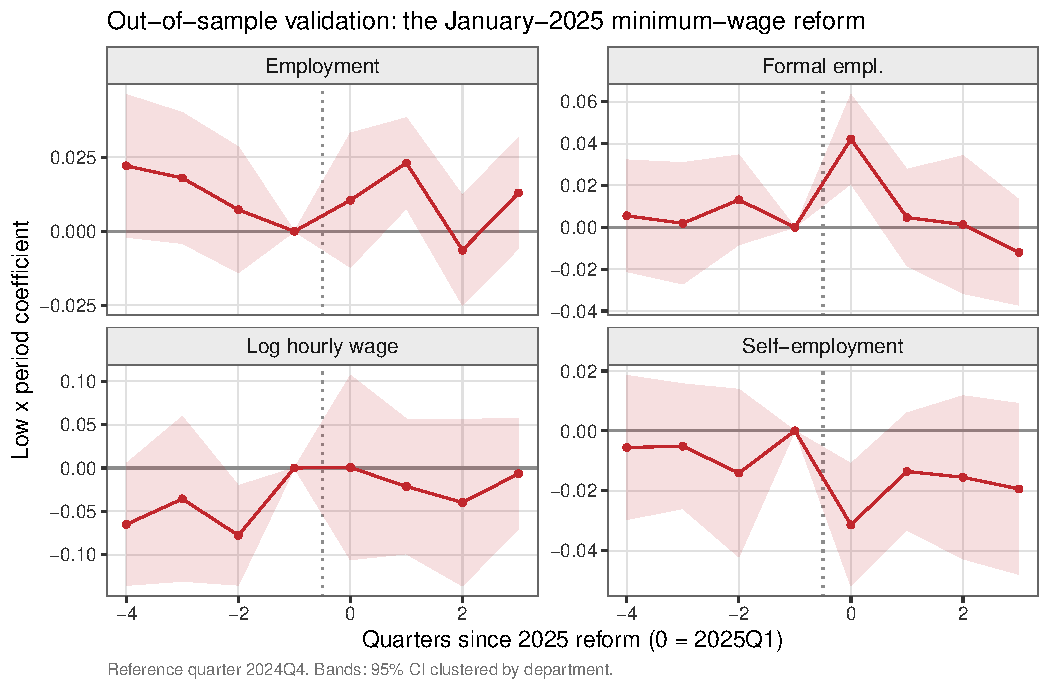
\includegraphics[width=0.9\textwidth]{fig9_validation2025.pdf}
\caption{Event study around the January-2025 reform (out-of-sample validation). Coefficients
on the interaction of the low-skill indicator with quarter indicators, reference quarter
2024Q4. Bands are ninety-five percent confidence intervals clustered by department.}
\label{fig:val2025}
\end{figure}

\begin{table}[!tbp]\centering
\caption{In-time placebo reforms (pre-reform window only)}\label{tab:placebo}
\begin{threeparttable}
\begin{tabular}{lccc}
\toprule
Outcome & Placebo 2021Q2 & Placebo 2021Q3 & Placebo 2021Q4 \\
\midrule
Log real hourly wage & 0.020 & -0.018 & -0.005 \\
 & (0.037) & (0.032) & (0.021) \\
Employment & -0.057$^{***}$ & -0.034$^{***}$ & -0.026$^{***}$ \\
 & (0.016) & (0.007) & (0.008) \\
Formal employment & -0.021$^{*}$ & -0.012 & -0.005 \\
 & (0.011) & (0.013) & (0.007) \\
Self-employment & 0.022$^{*}$ & -0.009 & 0.007 \\
 & (0.012) & (0.007) & (0.009) \\
\bottomrule
\end{tabular}

\begin{tablenotes}\footnotesize
\item Notes: Each entry is the $\mathrm{Low}\times\mathrm{Post}$ coefficient from a placebo
DiD that assigns a fake reform to the indicated quarter, estimated using only pre-reform
data (2021Q1--2022Q1). Standard errors clustered by department in parentheses; all estimates
are weighted by ENAHO survey weights. $^{*}p<0.1$, $^{**}p<0.05$, $^{***}p<0.01$.
\end{tablenotes}
\end{threeparttable}
\end{table}


\end{document}
